\documentclass[usenames, xcolor=dvipsnames]{beamer}
%% \documentclass[professionalfonts, xcolor=table, handout]{beamer}
%% \usepackage{pgfpages}
%% \pgfpagesuselayout{4 on 1}[a4paper,border shrink=5mm, landscape]
\usepackage{fontspec}
\usepackage{amsmath,amssymb}
\usepackage{pifont}% http://ctan.org/pkg/pifont
\usepackage{tikz}
\usetikzlibrary{positioning, matrix, arrows.meta, shapes.geometric, calc,
  decorations.pathmorphing, decorations.pathreplacing, fit, shapes.multipart}
\usepackage{mathabx}
\usepackage{mathtools}
\usepackage{mathpartir}
\usepackage{fancyvrb}
\usepackage{stmaryrd}
\usepackage[absolute,overlay]{textpos}
\usepackage[export]{adjustbox} % for subfigures

\definecolor{lightg}{RGB}{217,232,225}
\definecolor{darkg}{RGB}{6,81,42}
\definecolor{myred}{rgb}{0.0, 0.42, 0.24}
\colorlet{mypink}{myred!50!white}
\definecolor{mymaroon}{rgb}{0.86, 0.08, 0.24}

\defaultfontfeatures{Mapping=tex-text,Scale=MatchLowercase}
% \setmainfont{Libertinus Serif}
% \setsansfont{Libertinus Sans}
% \setmonofont{Menlo Regular}
\usetheme{Madrid}
\useoutertheme{infolines} % Alternatively: miniframes, infolines, split
\useinnertheme{circles}

% \setbeamertemplate{enumerate item}[default]
\usecolortheme[named=myred]{structure}
% \usecolortheme{spruce}
\usefonttheme{serif}
\setbeamerfont*{frametitle}{series=\bfseries}
\setbeamercolor{alerted text}{fg=mymaroon}
\setbeamertemplate{navigation symbols}{}
\setbeamercolor{emphC}{fg=myred}
% \setbeamercolor{block title}{bg = darkg, fg=white!80}
% \setbeamercolor{block body}{bg = lightg, fg=black}
\setbeamercolor{itemize item}{fg=black}
\setbeamercolor{description item}{fg=myred}

\newcommand{\sz}{\texttt{size}}
\newcommand{\ifty}{\texttt{inf}}
\newcommand{\scon}{\mathbin{\ast}}
\usepackage{scalerel}
\renewcommand{\bigstar}{\raisebox{-0.24em}{{\scaleobj{2.5}{\scon}}}}

\newcommand{\ocon}{%
  \mathbin{\mbox{$\mathrlap{\cup}\hspace*{.15em}
      \raisebox{.01em}[0ex][0ex]{$\scon$}$\hspace*{.07em}}}}
\newcommand{\medocon}{
  \raisebox{-0.3ex}{\resizebox{0.63em}{!}{$\scon$}} \hspace{-2.4ex} \bigcup}
\newcommand{\wand}{%
 \mathrel{\mbox{$\hspace*{-0.03em}\mathord{-}\hspace*{-0.66em}
  \mathord{-}\hspace*{-0.36em}\mathord{\scon}$\hspace*{-0.005em}}}}
\newcommand{\defeq}{\mathbin{\overset{\mathrm{def}}{=}}}
\newcommand{\emphd}[1]{{\bfseries #1}}
\newcommand{\emphr}[2]{\alert<#1>{#2}}
\newcommand{\bracket}[1]{[#1]}
\newcommand{\hide}[1]{}
\newcommand{\braces}[1]{\color{OliveGreen}\left\{\begin{array}{l@{}} \!\!\! #1 \end{array}\right\}}

\makeatletter\let\frametextheight\beamer@frametextheight\makeatother
\newcommand\credit[1]{%
  \begin{textblock*}{\paperwidth}(0pt,\textheight)
    \raggedleft #1\hspace{.5em}
\end{textblock*}}
\newcommand{\pguards}[1]{\llbracket #1 \rrbracket}
\newcommand{\xmark}{\ding{55}}%
\newcommand{\cmark}{\ding{51}}%
\newcommand{\m}[1]{\ensuremath{\mathit{#1}}} % math font
\newcommand{\p}[1]{\ensuremath{\mathsf{#1}}} % predicate font
\newcommand{\bi}{\Leftrightarrow} % equivalence of expressions


\title[Expanding CertiGraph]{Expanding CertiGraph: Dijkstra, Prim, and Kruskal}
\author[Mohan, Leow, Hobor]{\underline{Anshuman Mohan}, Wei Xiang Leow, Aquinas Hobor}
%\institute[NUS]{
\includegraphics[height=0.12\textwidth]{NUS_logo_full-horizontal.jpg}}
  \date[Cornell PLDG]{Cornell PLDG \\ \today}

\begin{document}
\begin{frame}[plain]
  \titlepage
\end{frame}

\begin{frame}{Saluting the Mothership}

\includegraphics[scale=0.09]{vst_logo}
\hspace{2em} 
\includegraphics[scale=0.12]{compcert_logo}
\hspace{2em} 
\includegraphics[scale=0.2]{paper_screen}

\bigskip
VST + CompCert + \underline{CertiGraph}

\bigskip
A Coq library to verify executable code
\\\hspace{1em}against realistic specifications
\\\hspace{2em}expressed with mathematical graphs

\end{frame}

\begin{frame}{This Work}

\includegraphics[scale=0.09]{vst_logo}
\hspace{2em} 
\includegraphics[scale=0.12]{compcert_logo}
\hspace{2em} 
\includegraphics[scale=0.2]{paper_screen}

\bigskip

We verify Dijkstra, Prim, Kruskal

\bigskip \pause

In doing so, we:
\\ \hspace{1em} Test existing features [Dijk labels edges]
\\ \hspace{1em} Expand into undirectedness [Prim, Krus]
\\ \hspace{1em} Make nontrivial calls to verified methods [Krus calls UF]

\end{frame}

\begin{frame}{Challenges}

Using CompCert C, which 
\\ \hspace{1em} is executable and realistic 
\\ \hspace{1em} but has real-world complications

\bigskip

Aiming for full functional correctness

\bigskip

Maintaining modularity and reuse
\end{frame}

\begin{frame}{Workflow}
    
\begin{tikzpicture}[remember picture,overlay, on grid,
      ourlib/.style={rounded corners=4pt, line width=0.8pt},
      cmd/.style={rectangle, fill=yellow!50!white, draw=black, rounded corners=4pt},
      file/.style={rounded corners=2pt, line width=1pt, fill=yellow!50!white},
      ->/.style={-Stealth, line width=1pt}]
    \path
    coordinate (nw) at ($(current page.north west) + (0.25, -1.5)$)
    coordinate (ne) at ($(current page.north east) + (-0.25, -1.5)$)
    coordinate (sw) at ($(current page.south west) + (0.25, 0.5)$)
    coordinate (se) at ($(current page.south east) + (-0.25, 0.5)$)
    coordinate (cright) at ($(current page.south west) + (2.85, 0.5)$)
    coordinate (asmleft) at ($(current page.south east) + (-2.85, 0.5)$)
    coordinate (coqleft) at ($(current page.south west)!.5!(current page.south east) +
    (-0.5, 0.5)$)
    coordinate (coqright) at ($(current page.south west)!.5!(current page.south east) +
    (0.5, 0.5)$);
    \draw [ourlib, fill=green!20!white] (nw) rectangle ($(sw) + (0.8, 0)$);
    \node at ($(nw)!.5!(sw) + (0.4, 0)$)
          {\rotatebox{-90}{\textsf{Mathematical Graph Library}}};
    \draw [ourlib, fill=red!20!white] (ne) rectangle ($(se) + (-0.8, 0)$);
    \node at ($(ne)!.5!(se) + (-0.4, 0)$)
          {\rotatebox{-90}{\textsf{Verified Software Toolchain (VST)}}};
    \draw [ourlib, fill=green!20!white] ($(nw) + (1.6, 0)$) rectangle
    ($(ne) + (-1.6, -0.8)$);
    \node at ($(nw)!.5!(ne) + (0, -0.4)$) {\textsf{Spatial Graph Library}};

    \draw [ourlib, fill=green!20!white] ($(nw) + (1.6, -1.6)$) -- ++(0, -0.8) --
    ++(1.6, 0) -- ++(0, -0.8) -- ++(-1.6, 0) -- ++(0, -0.8) -- ++(3.6, 0) --
    ++(0, 0.8) -- ++(-1.6, 0) -- ++(0, 0.8) -- ++(2, 0) -- ++(0, -0.5) -- ++(-1.6, 0)
    -- ++(0, -1.4) -- ++(3.6, 0) -- ++(0, 1.4) -- ++(-1.6, 0) -- ++(0, 0.5) -- ++(2, 0)
    -- ++(0, -0.8) -- ++(-1.6, 0) -- ++(0, -0.8) -- ++(4.2, 0) -- ++(0, 0.8) --
    ++(-1.6, 0) -- ++(0, 0.8) -- ($(ne) + (-1.6, -2.4)$) -- ++(0, 0.8) -- cycle;
    \node at ($(nw)!.5!(ne) + (0, -2)$)
          {\textsf{Verification of a Graph-Manipulating Function}};
    \draw [ourlib, fill=red!20!white] ($(sw) + (1.6, 0)$) -- ++(0, 0.8) --
    ($(cright) + (0.6, 0.8)$) -- ++(0, 1.8) -- ($(coqleft) + (-0.6, 2.6)$) --
    ++(0, -1.8) -- ($(coqright) + (0.6, 0.8)$) -- ++(0, 1.8) --
    ($(asmleft) + (-0.6, 2.6)$) -- ++(0, -1.8) -- ($(se) + (-1.6, 0.8)$) --
    ++(0, -0.8) -- cycle;
    \node at ($(sw)!.5!(se) + (0, 0.4)$) {\textsf{The CompCert Project}};
    \node (P0) at ($(nw) + (2.2, -3.6)$) {$\{P_0\}$};
    \node (C1) [cmd, right=1.2 of P0] {$C_1$};
    \node (P1) [right=2.4 of P0] {$\{P_1\}$};
    \node (P2) [right=2.4 of P1] {$\{P_2\}$};
    \node (P3) [right=2.8 of P2] {$\{...P_n\}$};
    \node (C2) [cmd, right=2.4 of C1] {$C_2$};
    \node (C3) [cmd, right=2.8 of C2] {$...C_n$};
    \draw [file] ($(sw)!.5!(se) + (-0.5, 1.2)$) -- ++(1, 0) -- ++ (0, 1.1) --
    +(-0.3, 0.3) -- +(-1, 0.3) -- cycle ++(1, 1.1) -- ++(-0.3, 0) -- ++(0, 0.3);
    \node at ($(sw)!.5!(se) + (0, 1.9)$) {\textsf{Coq}};
    \draw [file] ($(sw) + (1.6, 1.2)$) -- ++(1, 0) -- ++ (0, 1.1) --
    +(-0.3, 0.3) -- +(-1, 0.3) -- cycle ++(1, 1.1) -- ++(-0.3, 0) -- ++(0, 0.3);
    \node at ($(sw) + (2.1, 1.9)$) {\textsf{C}};
    \draw [file] ($(se) + (-2.6, 1.2)$) -- ++(1, 0) -- ++ (0, 1.1) --
    +(-0.3, 0.3) -- +(-1, 0.3) -- cycle ++(1, 1.1) -- ++(-0.3, 0) -- ++(0, 0.3);
    \node at ($(se) + (-2.1, 1.9)$) {\textsf{Asm}};
    \draw [->, dashed] ($(sw)!.5!(se) + (-0.3, 2.6)$) .. controls ++(-0.3, 0.5) and
    ($(C1.south) + (0.3, -1)$) .. (C1.south);
    \draw [->, dashed] ($(sw)!.5!(se) + (-0.2, 2.6)$) -- (C2.south);
    \draw [->, dashed] ($(sw)!.5!(se) + (-0.1, 2.6)$) .. controls ++(0.3, 0.5) and
    ($(C3.south) + (-0.3, -1)$) .. (C3.south);
    \node at ($(cright)!.5!(coqleft) + (0, 1.9)$) {\begin{tabular}{c} \textsf{Parser,}
        \\ \textsf{Simplifier} \end{tabular}};
    \node at ($(coqright)!.5!(asmleft) + (0, 1.9)$) {\begin{tabular}{c}
        \textsf{Verified} \\ \textsf{Compiler} \end{tabular}};
    \draw [->] ($(cright) + (0, 1.9)$) -- ++(0.6, 0);
    \draw [->] ($(coqleft) + (-0.6, 1.9)$) -- ++(0.6, 0);
    \draw [->] ($(coqright) + (0, 1.9)$) -- ++(0.6, 0);
    \draw [->] ($(asmleft) + (-0.6, 1.9)$) -- ++(0.6, 0);

    %% left interface
    \draw [line width=2pt] ($(nw) + (1.8, -0.4)$) -- +(-0.4, 0) +(-0.7, 0) --
    +(-1.2, 0) +(-0.6, -0.2) arc [start angle=-90, end angle=90, radius=0.2];
    \fill ($(nw) + (1.2, -0.4)$) circle [radius=0.1];
    \draw [line width=2pt] ($(nw) + (1.8, -2)$) -- +(-0.4, 0) +(-0.7, 0) --
    +(-1.2, 0) +(-0.6, -0.2) arc [start angle=-90, end angle=90, radius=0.2];
    \fill ($(nw) + (1.2, -2)$) circle [radius=0.1];

    %% right interface
    \draw [line width=2pt] ($(ne) + (-1.8, -2)$) -- +(0.4, 0) +(0.7, 0) --
    +(1.2, 0) +(0.6, 0.2) arc [start angle=90, end angle=270, radius=0.2];
    \fill ($(ne) + (-1.2, -2)$) circle [radius=0.1];
    \draw [line width=2pt] ($(se) + (-0.6, 0.4)$) -- +(-0.4, 0) +(-0.7, 0) --
    +(-1.2, 0) +(-0.6, -0.2) arc [start angle=-90, end angle=90, radius=0.2];
    \fill ($(se) + (-1.2, 0.4)$) circle [radius=0.1]; 
    
    %% up interface
    \draw [line width=2pt] ($(ne)!.5!(nw) + (2, -1.8)$) -- +(0, 0.4) +(0, 0.7) --
    +(0, 1.2) +(0.2, 0.6) arc [start angle=0, end angle=-180, radius=0.2];
    \fill ($(ne)!.5!(nw) + (2, -1.2)$) circle [radius=0.1];
  \end{tikzpicture}
\end{frame}


\subsection{Math Graph Architecture}
\begin{frame}{Math Graph Architecture}
  \centering
  \colorbox{lightg}{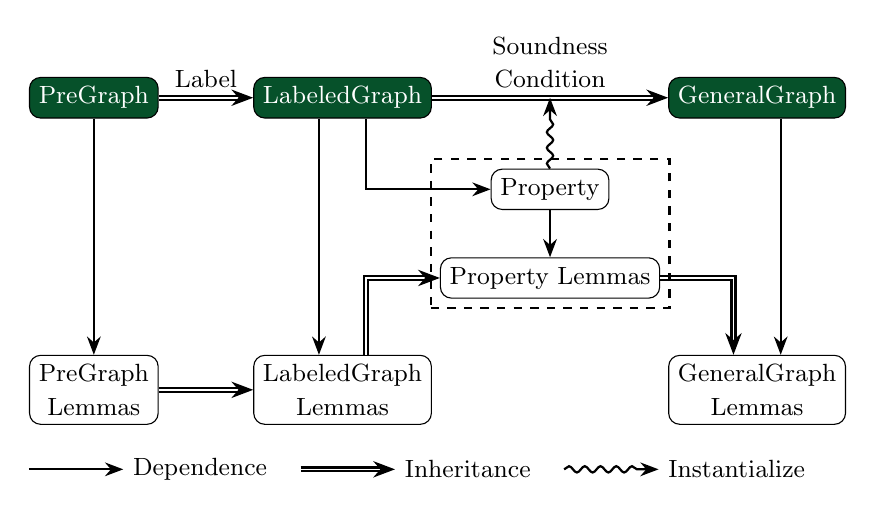
\begin{tikzpicture}
[->/.style={thick,arrows={-Stealth}},
-->/.style={thick,arrows={-Stealth}, decorate, decoration={snake, amplitude=.4mm,segment length=2mm,post length=2mm}},
   realG/.style={shape=rectangle, rounded corners=4pt, draw, fill=darkg},
   propG/.style={shape=rectangle, rounded corners=4pt, draw},
   x=1.5cm, y=1.5cm]
\node[realG] (PG) at (0, 0) {\small\color{white} PreGraph};
\node[realG] (LG) [right=0.8 of PG] {\small\color{white} LabeledGraph};
\node[realG] (GG) [right=2 of LG] {\small\color{white} GeneralGraph};
\draw [double, ->] (PG) -- (LG) node [pos=0.5, above] {\small Label} ;
\draw [double, ->] (LG) -- (GG) node (SC) [pos=0.5, above, align=center]
{\small Soundness \\ \small Condition};
\node[propG] (Prop) [below=0.6 of SC] {\small Property};
\node[propG] (PropL) [below=0.4 of Prop] {\small Property Lemmas};
\node[propG] (PGL) [below=2 of PG, align=center] {\small PreGraph \\\small Lemmas};
\node[propG] (LGL) [below=2 of LG, align=center] {\small LabeledGraph \\\small Lemmas};
\node[propG] (GGL) [below=2 of GG, align=center] {\small GeneralGraph \\\small Lemmas};
\draw [double, ->] (PGL) to (LGL);
%% \draw [double, ->] (LGL) to (GGL);
\draw [->] (PG) to (PGL);
\draw [->] (Prop) to (PropL);
\draw [-->] (Prop) to (SC);
\coordinate [left=0.2 of LG.south] (LGs1);
\coordinate [left=0.2 of LGL.north] (LGLn1);
\draw [->] (LGs1) to (LGLn1);
\coordinate [right=0.2 of LG.south] (LGs2);
\coordinate [right=0.2 of LGL.north] (LGLn2);
\draw [->] (LGs2) |- (Prop);
\draw [double, ->] (LGLn2) |- (PropL);
\coordinate [right=0.2 of GG.south] (GGs);
\coordinate [left=0.2 of GGL.north] (GGLn1);
\coordinate [right=0.2 of GGL.north] (GGLn2);
\draw [double, ->] (PropL) -| (GGLn1);
\draw [->] (GGs) to (GGLn2);
\node [draw, thick, rectangle, dashed, fit=(Prop) (PropL)] {};
\node (legend1) [below right=0.2 and -0.3 of PGL] {\small Dependence};
\coordinate[left=0.8 of legend1]  (l1);
\draw [->] (l1) to (legend1);
\node (legend2) [right=1 of legend1] {\small Inheritance};
\coordinate[left=0.8 of legend2]  (l2);
\draw [double, ->] (l2) to (legend2);
\node (legend3) [right=1 of legend2] {\small Instantialize};
\coordinate[left=0.8 of legend3]  (l3);
\draw [-->] (l3) to (legend3);
\end{tikzpicture}
}
\end{frame}

\begin{frame}{Instantiating DijkGraph}
A PreGraph is a hextuple (\texttt{VType}, \texttt{EType}, \texttt{vvalid}, \texttt{evalid}, \texttt{src}, \texttt{dst})
\vspace{-1.5em}
\begin{flushleft}
\begin{equation*}
\begin{split}
\textbf{Dijk\_PG($\gamma$) $\defeq$ \null} & \texttt{VType := Z} \\
                    &\texttt{EType := VType * VType} \\
                    &\texttt{src := fst} \\
                    &\texttt{dst := snd} \\ 
                    &\forall \m{v}.~\texttt{vvalid}(\gamma, \m{v}) \bi 0 \le \m{v} < {\sz} \\
                    &\forall \m{s,d}.~\texttt{evalid}(\gamma, \m{(s,d)}) \bi \texttt{vvalid}(\gamma, \m{s}) \wedge \texttt{vvalid}(\gamma, \m{d})
\end{split}
\end{equation*}
\end{flushleft}
\end{frame}

\begin{frame}[fragile]{Instantiating DijkGraph}
A LabeledGraph is a quadruple (PreGraph, \texttt{VL}, \texttt{EL}, \texttt{GL})
\vspace{-1.5em}
\begin{flushleft}
\begin{equation*}
\begin{split}
\textbf{Dijk\_LG($\gamma$) $\defeq$ \null} &\text{Dijk\_PG as shown} \\
                  &\texttt{VL := list EL} \\
                  &\texttt{EL := Z} \\
                  &\texttt{GL := unit} 
\end{split}
\end{equation*}
\end{flushleft}
\end{frame}

\begin{frame}[fragile]{Instantiating DijkGraph}
A GeneralGraph adds arbitrary soundness conditions
\vspace{-1.5em}
\begin{flushleft}
\begin{equation*}
\begin{split}
\textbf{DijkGraph($\gamma$) $\defeq$ \null} &\text{Dijk\_LG as shown, and } \\
                    &FiniteGraph(\gamma) \wedge \null \\
                    &\forall \m{i,j}.~\texttt{vvalid}(\gamma, \m{i}) \wedge \texttt{vvalid}(\gamma, \m{j}) \Rightarrow \\
                    &\qquad \m{i} = \m{j} \Rightarrow \texttt{elabel}(\gamma,(\m{i},{j})) = 0 \wedge \null \\
                    &\qquad \m{i} \neq \m{j} \Rightarrow 0 \le \texttt{elabel}(\gamma,(\m{i},{j})) \le \alert<2>{\lfloor \texttt{MAX/size} \rfloor} \wedge \null \\
                    &\cdots
\end{split}
\end{equation*}
\end{flushleft}
\end{frame}

\begin{frame}{Representing DijkGraph in Memory}
\begin{equation*}
\begin{split}
\p{list\_rep}(\gamma, \m{i}) &\defeq \texttt{data\_at  array  graph2mat}(\gamma)[\m{i}] \texttt{  list\_addr}(\gamma, \m{i}) \\
\vspace{1em}
\p{graph\_rep}(\gamma) &\defeq \underset{\texttt{vvalid}(\gamma,\m{v})}{\bigstar} \m{v}  \mapsto\p{list\_rep}(\gamma, \m{v})
\end{split}
\end{equation*}

\bigskip

\pause 
\quad Relies on restrictions placed at the Math level

\end{frame}

\begin{frame}[fragile]{Code and Specification}

\begin{Verbatim}
void dijkstra (int **graph, int src, int *dist, 
               int *prev, int size, int inf {
\end{Verbatim}
$\braces{\p{AdjMat}(\gamma) *
\mathsf{array}(\texttt{dist}, \_) * \mathsf{array}(\texttt{prev}, \_)}$
\pause
\begin{Verbatim}
 int pq = init(size); int i, j, u, cost;
 for (i = 0; i < size; i++)
 {  dist[i] = inf; prev[i] = inf; push(i, inf, pq);  }
 dist[src] = 0; prev[src] = src; dec_key(src, 0, pq);
\end{Verbatim}
\pause
$\braces{{\color{mymaroon}\exists \m{dist}, \m{prev}, \m{popped}}.~\p{AdjMat}(\gamma) * {\color{mymaroon}\p{PQ}(\texttt{pq})} * \mathsf{array}(\texttt{dist},{\color{mymaroon}\m{dist}}) * \null \\ \mathsf{array}(\texttt{prev}, {\color{mymaroon}\m{prev}}) \wedge
{\color{mymaroon}\m{dijk\_correct}(\gamma,\texttt{src},\m{popped},\m{prev},\m{dist})}}$
\begin{Verbatim}
 // big while loop
\end{Verbatim}
\end{frame}

\begin{frame}[fragile]{Code and Specification}
$\braces{\exists \m{dist}, \m{prev}, \m{popped}.~\p{AdjMat}(\gamma) * \p{PQ}(\texttt{pq}) * \mathsf{array}(\texttt{dist},\m{dist}) * \null \\ \mathsf{array}(\texttt{prev}, \m{prev}) \wedge
\m{dijk\_correct}(\gamma,\texttt{src},\m{popped},\m{prev},\m{dist})}$
\pause
\begin{Verbatim}
 while (!pq_emp(pq)) {
  u = popMin(pq);
\end{Verbatim}
\pause 
$\color{OliveGreen}//~\braces{{\color{mymaroon}\exists \m{dist'}, \m{prev'}, \m{popped'}, \m{i}}.~\p{AdjMat}(\gamma) * \p{PQ}(\texttt{pq}) * \null \\
\mathsf{array}(\texttt{dist},\m{\color{mymaroon}dist'}) * \mathsf{array}(\texttt{prev}, \m{\color{mymaroon}prev'}) \wedge \null \\
{\color{mymaroon}\m{dijk\_correct\_weak}(\gamma, \texttt{src}, \m{popped'}, \m{prev'}, \m{dist'}, \m{i}, \texttt{u})}}$
\pause
\begin{Verbatim}
  for (i = 0; i < size; i++) {
  cost = getCell(graph, u, i);
  if (cost < inf) {
   if (dist[i] > dist[u] + cost) {
    dist[i] = dist[u] + cost; prev[i] = u;
    dec_key(i, dist[i], pq); 
 }}} // for
\end{Verbatim}
\pause
$\braces{{\color{mymaroon}\exists \m{dist''}, \m{prev''}}.~\p{AdjMat}(\gamma) * \p{PQ}(\texttt{pq}) *
  \mathsf{array}(\texttt{dist},\m{\color{mymaroon}dist''}) * \null \\
  \mathsf{array}(\texttt{prev}, \m{\color{mymaroon}prev''}) \wedge
  {\color{mymaroon}\m{dijk\_correct}(\gamma, \texttt{src}, \m{popped'}, \m{prev''}, \m{dist''})}}$
\end{frame}

\begin{frame}[fragile]{Code and Specification}
$\braces{\exists \m{dist}, \m{prev}, \m{popped}.~\p{AdjMat}(\gamma) * \p{PQ}(\texttt{pq}) * \mathsf{array}(\texttt{dist},\m{dist}) * \null \\ \mathsf{array}(\texttt{prev}, \m{prev}) \wedge
\m{dijk\_correct}(\gamma,\texttt{src},\m{popped},\m{prev},\m{dist})}$
\begin{Verbatim}
 while (!pq_emp(pq)) {
  u = popMin(pq);
  for (i = 0; i < size; i++) {
  cost = getCell(graph, u, i);
  if (cost < inf) {
   if (dist[i] > dist[u] + cost) {
    dist[i] = dist[u] + cost; prev[i] = u;
    dec_key(i, dist[i], pq); 
  }}} // for
\end{Verbatim}
\pause
\begin{Verbatim}
 } // while
\end{Verbatim}
\pause
$\color{OliveGreen}//~\braces{{\color{mymaroon}\exists \m{dist^{\circ}}, \m{prev^{\circ}}, \m{popped^{\circ}}}.~\p{AdjMat}(\gamma) * \p{PQ}(\texttt{pq}) * \null \\
\mathsf{array}(\texttt{dist},\m{\color{mymaroon}dist^{\circ}}) * 
\mathsf{array}(\texttt{prev}, \m{\color{mymaroon}prev^{\circ}}) \wedge \null \\
{\color{mymaroon}\m{all\_popped(popped^{\circ})}} \wedge
{\color{mymaroon}\m{dijk\_correct}(\gamma,\texttt{src},\m{popped^{\circ}},\m{prev^{\circ}},\m{dist^{\circ}})}}$
\pause
\begin{Verbatim}
 freePQ (pq); return;
}
\end{Verbatim}
\end{frame}


\begin{frame}{dijk\_correct}

\begin{equation*}
\begin{split}
\m{dijk\_correct}(\gamma, \m{src}, &\m{popped}, \m{prev}, \m{dist}) \; \defeq \; \\
\forall \m{d}.~vvalid(\gamma, \m{d}) \Rightarrow \\
\alert<2>{\big( \m{d} \in \m{popped} \; \Rightarrow} \; & \\ 
& \hspace{-5em} \exists \m{path}.~\m{path\_correct}(\gamma, \m{prev}, \m{path}, \m{src}, \m{d}) \wedge \null \\
& \hspace{-5em} \m{path\_globally\_optimal}(\gamma, \m{dist}, \m{path}) \alert<2>{\big)} \wedge \null \\
\alert<3>{\big( \m{dist}[\m{d}] < \ifty \; \Rightarrow} \; & \\ 
& \hspace{-5em} \texttt{let }\m{m} \texttt{ := } \m{prev}[\m{d}] \texttt{ in } \m{m} \in \m{popped}(\m{priq}) \wedge \null \\
& \hspace{-5em} \forall \m{m'} \in \m{popped}(\m{priq}).~\m{cost}(\m{p2m} \texttt{+} (m, d)) \le \m{cost}(\m{p2m'} \texttt{+} (m', d)) \alert<3>{\big)} \wedge \null \\
\alert<4>{\big( \m{dist}[\m{d}] = \ifty \; \Rightarrow} \; & \\ 
& \hspace{-5em} \forall \m{m} \in \m{popped}(\m{priq}).~\m{cost}(\m{p2m} \texttt{+} (m, d)) = \ifty \alert<4>{\big)}
\end{split}
\end{equation*}

\end{frame}


\newcommand{\s}{11}
\begin{frame}{Key Transformation: Growing the Subgraph}

\begin{center}
\begin{adjustbox}{scale=0.50}
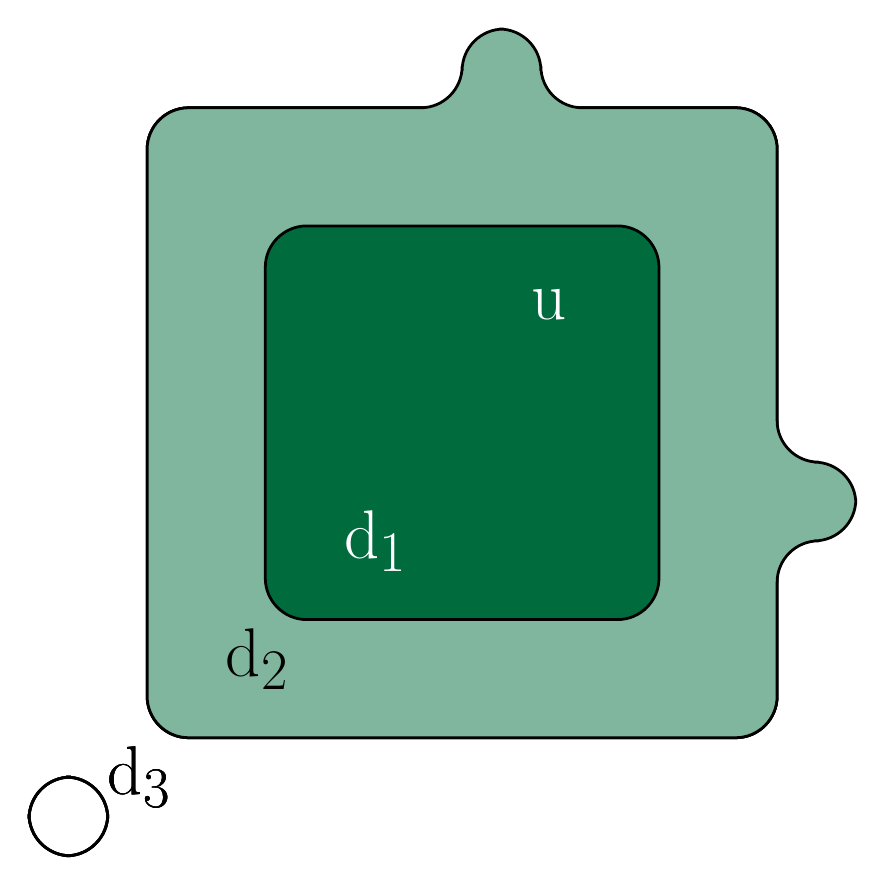
\begin{tikzpicture}[on grid,
  popped/.style={rounded corners=15pt, line width=1pt, draw, fill=myred},
  fringe/.style={rounded corners=15pt, line width=1pt, draw, fill=mypink},
  popping/.style={rounded corners=15pt, line width=1pt, draw, dashed, fill=mymaroon},
  unseen/.style={rounded corners=15pt, line width=1pt, draw}]
  \uncover<1>{
  \draw[unseen] (0,0) -- (\s,0) -- (\s,\s) -- (0,\s) -- cycle;
  \draw[fringe] (1.5,1.5) -- (9.5,1.5) -- (9.5,9.5) -- (1.5,9.5) -- cycle;
  \draw[popped] (3,3) -- (8,3) -- (6,6) -- (3,8) -- cycle;
  \node at (1.4,1) {\Huge d$_3$};   
  \node at (2.9,2.5) {\Huge d$_2$};   
  \node at (4.4,4) {\Huge \color{white}d$_1$}; 
  \node at (6.6,7) {\Huge u};}
  \uncover<2>{
    \draw[unseen] (0,0) -- (\s,0) -- (\s,\s) -- (0,\s) -- cycle;
  \draw[fringe] (1.5,1.5) -- (9.5,1.5) -- (9.5,9.5) -- (1.5,9.5) -- cycle;
  \draw[popping] (3,3) -- (8,3) -- (8,8) -- (3,8) -- cycle;
  \draw[popped] (3,3) -- (8,3) -- (6,6) -- (3,8) -- cycle;
  \node at (1.4,1) {\Huge d$_3$};   
  \node at (2.9,2.5) {\Huge d$_2$};   
  \node at (4.4,4) {\Huge \color{white}d$_1$}; 
  \node at (6.6,7) {\Huge u}; }
  \uncover<3>{
    \draw[unseen] (0,0) -- (\s,0) -- (\s,\s) -- (0,\s) -- cycle;
  \draw[fringe] (1.5,1.5) -- (9.5,1.5) -- (9.5, 4.0) -- (10.5, 4.0) -- (10.5, 5.0) -- (9.5, 5.0) -- (9.5,9.5) -- (6.5, 9.5) -- (6.5, 10.5) -- (5.5, 10.5) -- (5.5, 9.5) -- (1.5,9.5) -- cycle;
  \draw[popped] (3,3) -- (8,3) -- (8,8) -- (3,8) -- cycle;
  \node at (1.4,1) {\Huge d$_3$};   
  \node at (2.9,2.5) {\Huge d$_2$};   
  \node at (4.4,4) {\Huge \color{white}d$_1$}; 
  \node at (6.6,7) {\Huge \color{white}u}; }
\end{tikzpicture}
\end{adjustbox}
\end{center}
\end{frame}

\begin{frame}{dijk\_correct\_weak}

\begin{equation*}
\begin{split}
&\hspace{-1em}\m{dijk\_correct\_weak}(\gamma, \m{src}, \m{popped}, \m{prev}, \m{dist}, \m{i}, \m{u}) \; \defeq \; \forall \m{d}.~ \\
&\alert<2>{\big( vvalid(\gamma, \m{d}) \; \Rightarrow} \; \m{d} \in \m{popped} \; \Rightarrow \; \ldots \alert<2>{\big)} \wedge \\
&\alert<2>{\Big( 0 \le dst < i \; \Rightarrow} \; 
\big( \m{dist}[\m{d}] < \ifty \; \Rightarrow \ldots \big) \wedge
\big( \m{dist}[\m{d}] = \ifty \; \Rightarrow \ldots \big) \alert<2>{\Big)} \wedge \null \\
&\alert<3>{\Big( i \le dst < size \; \Rightarrow} \; \null \\
&\hspace{1em}\big( \m{dist}[\m{d}] < \ifty \; \Rightarrow \ldots \alert<4>{\wedge m \neq u \wedge m' \neq u} \big) \wedge \null \\
&\hspace{1em}\big( \m{dist}[\m{d}] = \ifty \; \Rightarrow \ldots \alert<4>{\wedge m \neq u} \big) \alert<3>{\Big)} \\
\end{split}
\end{equation*}

\end{frame}

\begin{frame}{Postcondition}

\begin{center}
\begin{adjustbox}{scale=0.50}
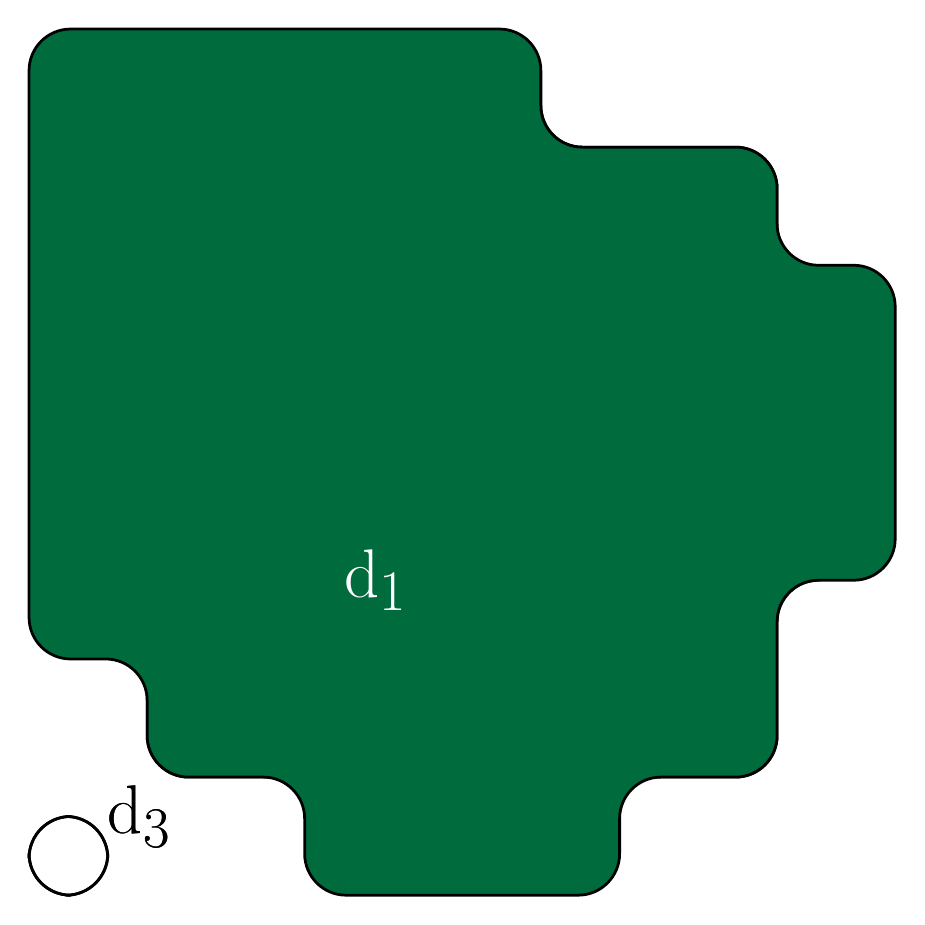
\begin{tikzpicture}[on grid,
  popped/.style={rounded corners=15pt, line width=1pt, draw, fill=myred},
  fringe/.style={rounded corners=15pt, line width=1pt, draw, fill=mypink},
  popping/.style={rounded corners=15pt, line width=1pt, draw, dashed, fill=mymaroon},
  unseen/.style={rounded corners=15pt, line width=1pt, draw}]
  \uncover<1>{
    \draw[unseen] (0,0) -- (\s,0) -- (\s,\s) -- (0,\s) -- cycle;
  \draw[fringe] (1.5,1.5) -- (9.5,1.5) -- (9.5, 4.0) -- (10.5, 4.0) -- (10.5, 5.0) -- (9.5, 5.0) -- (9.5,9.5) -- (6.5, 9.5) -- (6.5, 10.5) -- (5.5, 10.5) -- (5.5, 9.5) -- (1.5,9.5) -- cycle;
  \draw[popped] (3,3) -- (8,3) -- (8,8) -- (3,8) -- cycle;
  \node at (1.4,1) {\Huge d$_3$};   
  \node at (2.9,2.5) {\Huge d$_2$};   
  \node at (4.4,4) {\Huge \color{white}d$_1$}; }
  \uncover<2>{
    \draw[unseen] (0,0) -- (\s,0) -- (\s,\s) -- (0,\s) -- cycle;
  \draw[popped] (1.5,1.5) -- (3.5, 1.5) -- (3.5, 0) -- (7.5, 0) -- (7.5, 1.5) -- (9.5,1.5) -- (9.5, 4.0) -- (11, 4.0) -- (11, 8.0) -- (9.5, 8.0) -- (9.5,9.5) -- (6.5, 9.5) -- (6.5, 11) -- (0, 11) -- (0, 3) -- (1.5, 3) -- cycle;
  \node at (1.4,1) {\Huge d$_3$};   
  \node at (4.4,4) {\Huge \color{white}d$_1$}; } 
\end{tikzpicture}
\end{adjustbox}
\end{center}
\end{frame}

\begin{frame}{Overflow Strikes Again}

The longest optimal path has \texttt{size-1} links \\
\hspace{1em} \pause so say we set \texttt{elabel}'s upper bound to $\lfloor\texttt{MAX/(size-1)}\rfloor$ 

\bigskip \pause
\texttt{MAX} = 7, \texttt{size} = 3, so $0 \le \texttt{elabel}(\gamma, \m{e}) \le 3$.

\bigskip

{\centering
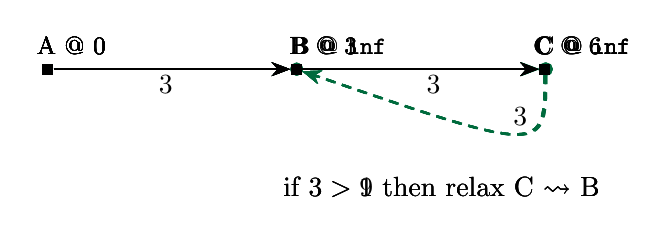
\begin{tikzpicture}
[vad/.style={rectangle, fill=black, inner sep=0pt, minimum size=4pt},
 inf/.style={circle, draw=myred, thick, inner sep=0pt, minimum size=4pt},
 inv/.style={circle, fill=myred, draw=myred, thick, inner sep=0pt, minimum size=4pt},
 ->/.style={thick, arrows={-Stealth}}]

  \node at (1.5,-0.2) {3};
  \node at (4.9,-0.2) {3};
  \node at (6,-0.6) {3};


\uncover<3>{
\node at (0.3, 0.3) {\small A @ 0};
\node at (3.7, 0.3) {\small B @ \ifty};
\node at (6.8, 0.3) {\small C @ \ifty}; 
  \node[vad] (A) at (0,0) {};
  \node[inf] (B) [right = 3 of A] {};
  \node[inf] (C) [right = 3 of B] {};
  \draw [->, dashed, myred] (A) -- (B);
  \draw [->, dashed, myred] (B) -- (C);
  \draw [->, dashed, myred] (C.south) .. controls ++(0, -1) .. (B);}
 
\uncover<4>{
\node at (0.3, 0.3) {\small A @ 0};
\node at (3.7, 0.3) {\small B @ \ifty};
\node at (6.8, 0.3) {\small C @ \ifty};  
  \node[vad] (A) at (0,0) {};
  \node[inv] (B) [right = 3 of A] {};
  \node[inf] (C) [right = 3 of B] {};
  \draw [->, dashed, myred] (A) -- (B);
  \draw [->, dashed, myred] (B) -- (C);
  \draw [->, dashed, myred] (C.south) .. controls ++(0, -1) .. (B);}

\uncover<5>{
\node at (0.3, 0.3) {\small A @ 0};
\node at (3.5, 0.3) {\small B @ 3};
\node at (6.8, 0.3) {\small C @ \ifty};  
  \node[vad] (A) at (0,0) {};
  \node[vad] (B) [right = 3 of A] {};
  \node[inf] (C) [right = 3 of B] {};
  \draw [->] (A) -- (B);
  \draw [->, dashed, myred] (B) -- (C);
  \draw [->, dashed, myred] (C.south) .. controls ++(0, -1) .. (B);
  }

\uncover<6>{ 
\node at (0.3, 0.3) {\small A @ 0};
\node at (3.5, 0.3) {\small B @ 3};
\node at (6.8, 0.3) {\small C @ \ifty};  
  \node[vad] (A) at (0,0) {};
  \node[vad] (B) [right = 3 of A] {};
  \node[inv] (C) [right = 3 of B] {};
  \draw [->] (A) -- (B);
  \draw [->, dashed, myred] (B) -- (C);
  \draw [->, dashed, myred] (C.south) .. controls ++(0, -1) .. (B);
}

\uncover<7>{ 
\node at (0.3, 0.3) {\small A @ 0};
\node at (3.5, 0.3) {\small B @ 3};
\node at (6.6, 0.3) {\small C @ 6};  
  \node[vad] (A) at (0,0) {};
  \node[vad] (B) [right = 3 of A] {};
  \node[vad] (C) [right = 3 of B] {};
  \draw [->] (A) -- (B);
  \draw [->] (B) -- (C);
  \draw [->, dashed, myred] (C.south) .. controls ++(0, -1) .. (B);
}

\uncover<8>{ 
\node at (0.3, 0.3) {\small A @ 0};
\node at (3.5, 0.3) {\small B @ 3};
\node at (6.6, 0.3) {\small C @ 6};  
\node at (5, -1.5) {if $3 > 9$ then relax C $\leadsto$ B};
  \node[vad] (A) at (0,0) {};
  \node[vad] (B) [right = 3 of A] {};
  \node[vad] (C) [right = 3 of B] {};
  \draw [->] (A) -- (B);
  \draw [->] (B) -- (C);
  \draw [->, dashed, myred] (C.south) .. controls ++(0, -1) .. (B);
}

\uncover<9>{ 
\node at (0.3, 0.3) {\small A @ 0};
\node at (3.5, 0.3) {\small B @ 3};
\node at (6.6, 0.3) {\small C @ 6};  
\node at (5, -1.5) {if $3 > \alert{1}$ then relax C $\leadsto$ B};
  \node[vad] (A) at (0,0) {};
  \node[vad] (B) [right = 3 of A] {};
  \node[vad] (C) [right = 3 of B] {};
  \draw [->] (A) -- (B);
  \draw [->] (B) -- (C);
  \draw [->, dashed, myred] (C.south) .. controls ++(0, -1) .. (B);
}

\uncover<10->{ 
\node at (0.3, 0.3) {\small A @ 0};
\node at (3.5, 0.3) {\small B @ \alert{1}};
\node at (6.6, 0.3) {\small C @ 6}; 
\node at (5, -1.5) {if $3 > 1$ then \alert{relax C $\leadsto$ B}};
  \node[vad] (A) at (0,0) {};
  \node[vad] (B) [right = 3 of A] {};
  \node[vad] (C) [right = 3 of B] {};
  \draw [->] (A) -- (B);
  \draw [->] (B) -- (C);
  \draw [->, dashed, myred] (C.south) .. controls ++(0, -1) .. (B);
}

\end{tikzpicture}

}

\bigskip

\uncover<11->{
One solution: Conservatively set upper bound to $\lfloor\texttt{MAX/size}\rfloor$}

\bigskip

\uncover<12->{
Max path cost is then  
$\lfloor\texttt{MAX/size}\rfloor$ \texttt{ * (size-1) = MAX - }$\lfloor\texttt{MAX/size}\rfloor$}
\end{frame}

\begin{frame}{Overflow Strikes Again}

There are other ways to fix this!
\\ \pause \hspace{1em} Refactor troublesome addition as subtraction
\\ \pause \hspace{1em} Never look back into optimized part
\\ \pause \hspace{1em} Your suggestion here
\\ \pause \hspace{1em} Your suggestion here

\bigskip

\pause Sadly, intuition supports \texttt{inf = MAX}

\end{frame}


\begin{frame}{Prim: Extending to Undirectedness}

Consider the AdjMat representation of a directed graph: \\
\centering
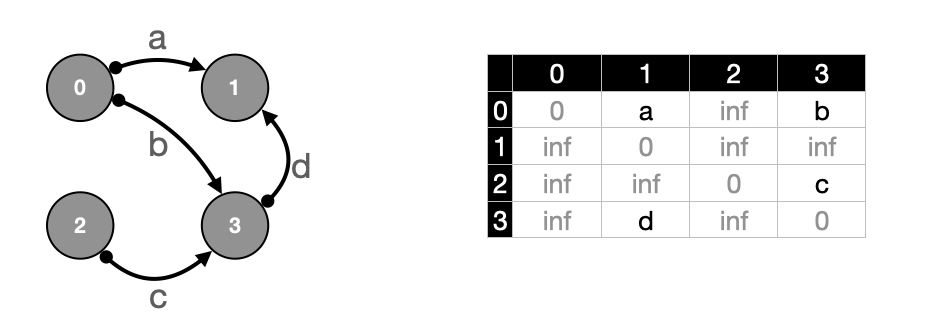
\includegraphics[scale=0.7]{directed}

\end{frame}

\begin{frame}{Prim: Extending to Undirectedness}

Versus the AdjMat representation of an undirected graph: \\
\centering
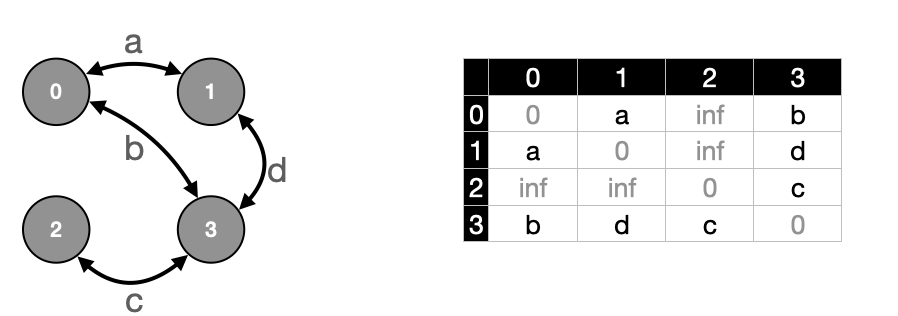
\includegraphics[scale=0.7]{undirected}

\end{frame}

\begin{frame}[fragile]{Prim: Extending to Undirectedness}

Prevent double-counting:
\begin{Verbatim}
Class SoundUAdjMat (g: UAdjMatLG) := {
  sadjmat: @SoundAdjMat size inf g;
  undirec: forall e, evalid g e -> src g e <= dst g e;
}.
\end{Verbatim}

\pause \bigskip
Build undirected idioms:
\begin{Verbatim}
Definition adj_edge g e u v :=
  ((src g e = u /\ dst g e = v) \/ 
   (src g e = v /\ dst g e = u)).
\end{Verbatim}
Plus \texttt{upath}, \texttt{connected}, \emph{etc.}
\end{frame}

\begin{frame}{Recall: Math Graph Architecture}
  \centering
  \colorbox{lightg}{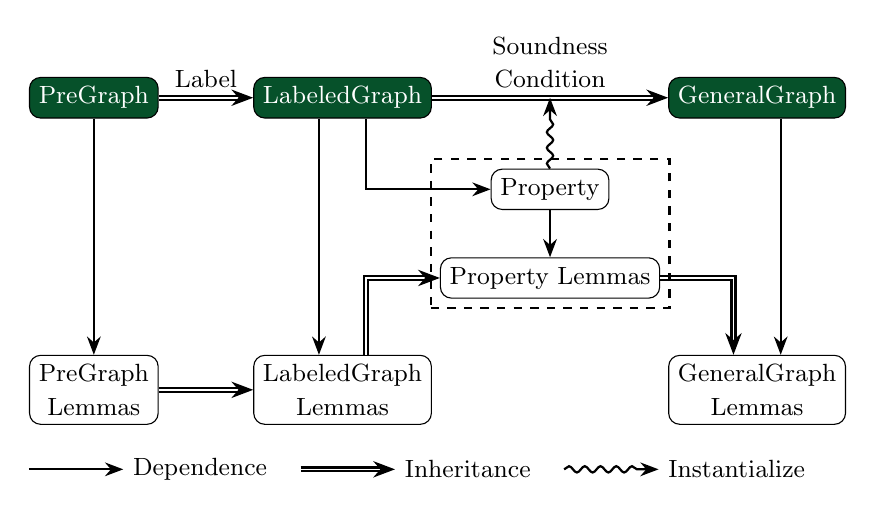
\begin{tikzpicture}
[->/.style={thick,arrows={-Stealth}},
-->/.style={thick,arrows={-Stealth}, decorate, decoration={snake, amplitude=.4mm,segment length=2mm,post length=2mm}},
   realG/.style={shape=rectangle, rounded corners=4pt, draw, fill=darkg},
   propG/.style={shape=rectangle, rounded corners=4pt, draw},
   x=1.5cm, y=1.5cm]
\node[realG] (PG) at (0, 0) {\small\color{white} PreGraph};
\node[realG] (LG) [right=0.8 of PG] {\small\color{white} LabeledGraph};
\node[realG] (GG) [right=2 of LG] {\small\color{white} GeneralGraph};
\draw [double, ->] (PG) -- (LG) node [pos=0.5, above] {\small Label} ;
\draw [double, ->] (LG) -- (GG) node (SC) [pos=0.5, above, align=center]
{\small Soundness \\ \small Condition};
\node[propG] (Prop) [below=0.6 of SC] {\small Property};
\node[propG] (PropL) [below=0.4 of Prop] {\small Property Lemmas};
\node[propG] (PGL) [below=2 of PG, align=center] {\small PreGraph \\\small Lemmas};
\node[propG] (LGL) [below=2 of LG, align=center] {\small LabeledGraph \\\small Lemmas};
\node[propG] (GGL) [below=2 of GG, align=center] {\small GeneralGraph \\\small Lemmas};
\draw [double, ->] (PGL) to (LGL);
%% \draw [double, ->] (LGL) to (GGL);
\draw [->] (PG) to (PGL);
\draw [->] (Prop) to (PropL);
\draw [-->] (Prop) to (SC);
\coordinate [left=0.2 of LG.south] (LGs1);
\coordinate [left=0.2 of LGL.north] (LGLn1);
\draw [->] (LGs1) to (LGLn1);
\coordinate [right=0.2 of LG.south] (LGs2);
\coordinate [right=0.2 of LGL.north] (LGLn2);
\draw [->] (LGs2) |- (Prop);
\draw [double, ->] (LGLn2) |- (PropL);
\coordinate [right=0.2 of GG.south] (GGs);
\coordinate [left=0.2 of GGL.north] (GGLn1);
\coordinate [right=0.2 of GGL.north] (GGLn2);
\draw [double, ->] (PropL) -| (GGLn1);
\draw [->] (GGs) to (GGLn2);
\node [draw, thick, rectangle, dashed, fit=(Prop) (PropL)] {};
\node (legend1) [below right=0.2 and -0.3 of PGL] {\small Dependence};
\coordinate[left=0.8 of legend1]  (l1);
\draw [->] (l1) to (legend1);
\node (legend2) [right=1 of legend1] {\small Inheritance};
\coordinate[left=0.8 of legend2]  (l2);
\draw [double, ->] (l2) to (legend2);
\node (legend3) [right=1 of legend2] {\small Instantialize};
\coordinate[left=0.8 of legend3]  (l3);
\draw [-->] (l3) to (legend3);
\end{tikzpicture}
}
\end{frame}

\begin{frame}{Kruskal: EdgeList Representation}
Extend spatial support to accommodate EdgeList representation

\bigskip

The double-counting restriction must be lifted: \\
\hspace{1em}an EdgeList-represented graph can have bona fide multi-connections

\bigskip

But the undirected idioms carry over
\end{frame}

\begin{frame}{Kruksal: Layering Undirectedness Atop Union-Find}
  Consider performing \texttt{union u w} \\
  Note: \texttt{reachable} is directed, \texttt{connected} is undirected \\
  \vspace{2em}
  \centering
  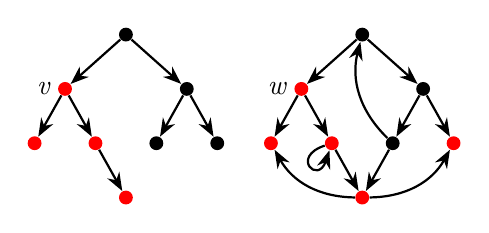
\begin{tikzpicture}[
  gnode/.style={circle, inner sep=0pt, minimum size=5pt, fill=black},
  gnodecol/.style={circle, inner sep=0pt, minimum size=5pt, fill=red},
  ->/.style={-Stealth, thick}, node distance=0.5cm]
  \node[gnode] (n0) {};
  \node[gnodecol] (n1) [below = of n0, xshift=-22pt] {};
  \node [left = of n1, xshift = 16pt] {$\m{v}$};
  \node[gnode] (n2) [below = of n0, xshift=22pt] {};
  \node[gnodecol] (n3) [below = of n1, xshift=-11pt] {};
  \node[gnodecol] (n4) [below = of n1, xshift=11pt] {};
  \node[gnode] (n5) [below = of n2, xshift=-11pt] {};
  \node[gnode] (n6) [below = of n2, xshift=11pt] {};
  \node[gnodecol] (n7) [below = of n4, xshift=11pt] {};
  \draw[->] (n0) to (n1);
  \draw[->] (n0) to (n2);
  \draw[->] (n1) to (n3);
  \draw[->] (n1) to (n4);
  \draw[->] (n2) to (n5);
  \draw[->] (n2) to (n6);
  \draw[->] (n4) to (n7);
  \node[gnode] (m0) [right = 80pt of n0]{};
  \node[gnodecol] (m1) [below = of m0, xshift=-22pt] {};
  \node [left = of m1, xshift = 16pt] {$\m{w}$};
  \node[gnode] (m2) [below = of m0, xshift=22pt] {};
  \node[gnodecol] (m3) [below = of m1, xshift=-11pt] {};
  \node[gnodecol] (m4) [below = of m1, xshift=11pt] {};
  \node[gnode] (m5) [below = of m2, xshift=-11pt] {};
  \node[gnodecol] (m6) [below = of m2, xshift=11pt] {};
  \node[gnodecol] (m7) [below = of m4, xshift=11pt] {};
  \draw[->] (m0) to (m1);
  \draw[->] (m0) to (m2);
  \draw[->] (m1) to (m3);
  \draw[->] (m1) to (m4);
  \draw[->] (m2) to (m5);
  \draw[->] (m2) to (m6);
  \draw[->] (m4) to (m7);
  \draw[->] (m5) to (m7);
  \draw[->] (m5) to [bend left] (m0);
  \draw[->] (m4) .. controls ([xshift=-15pt, yshift=-5pt] m4) and ([xshift=-5pt, yshift=-15pt] m4) .. (m4);
  \draw[->] (m7) to [bend right] (m6);
  \draw[->] (m7) to [bend left] (m3);
\end{tikzpicture}

\end{frame}

\begin{frame}{A Note on Modularity}
\centering
  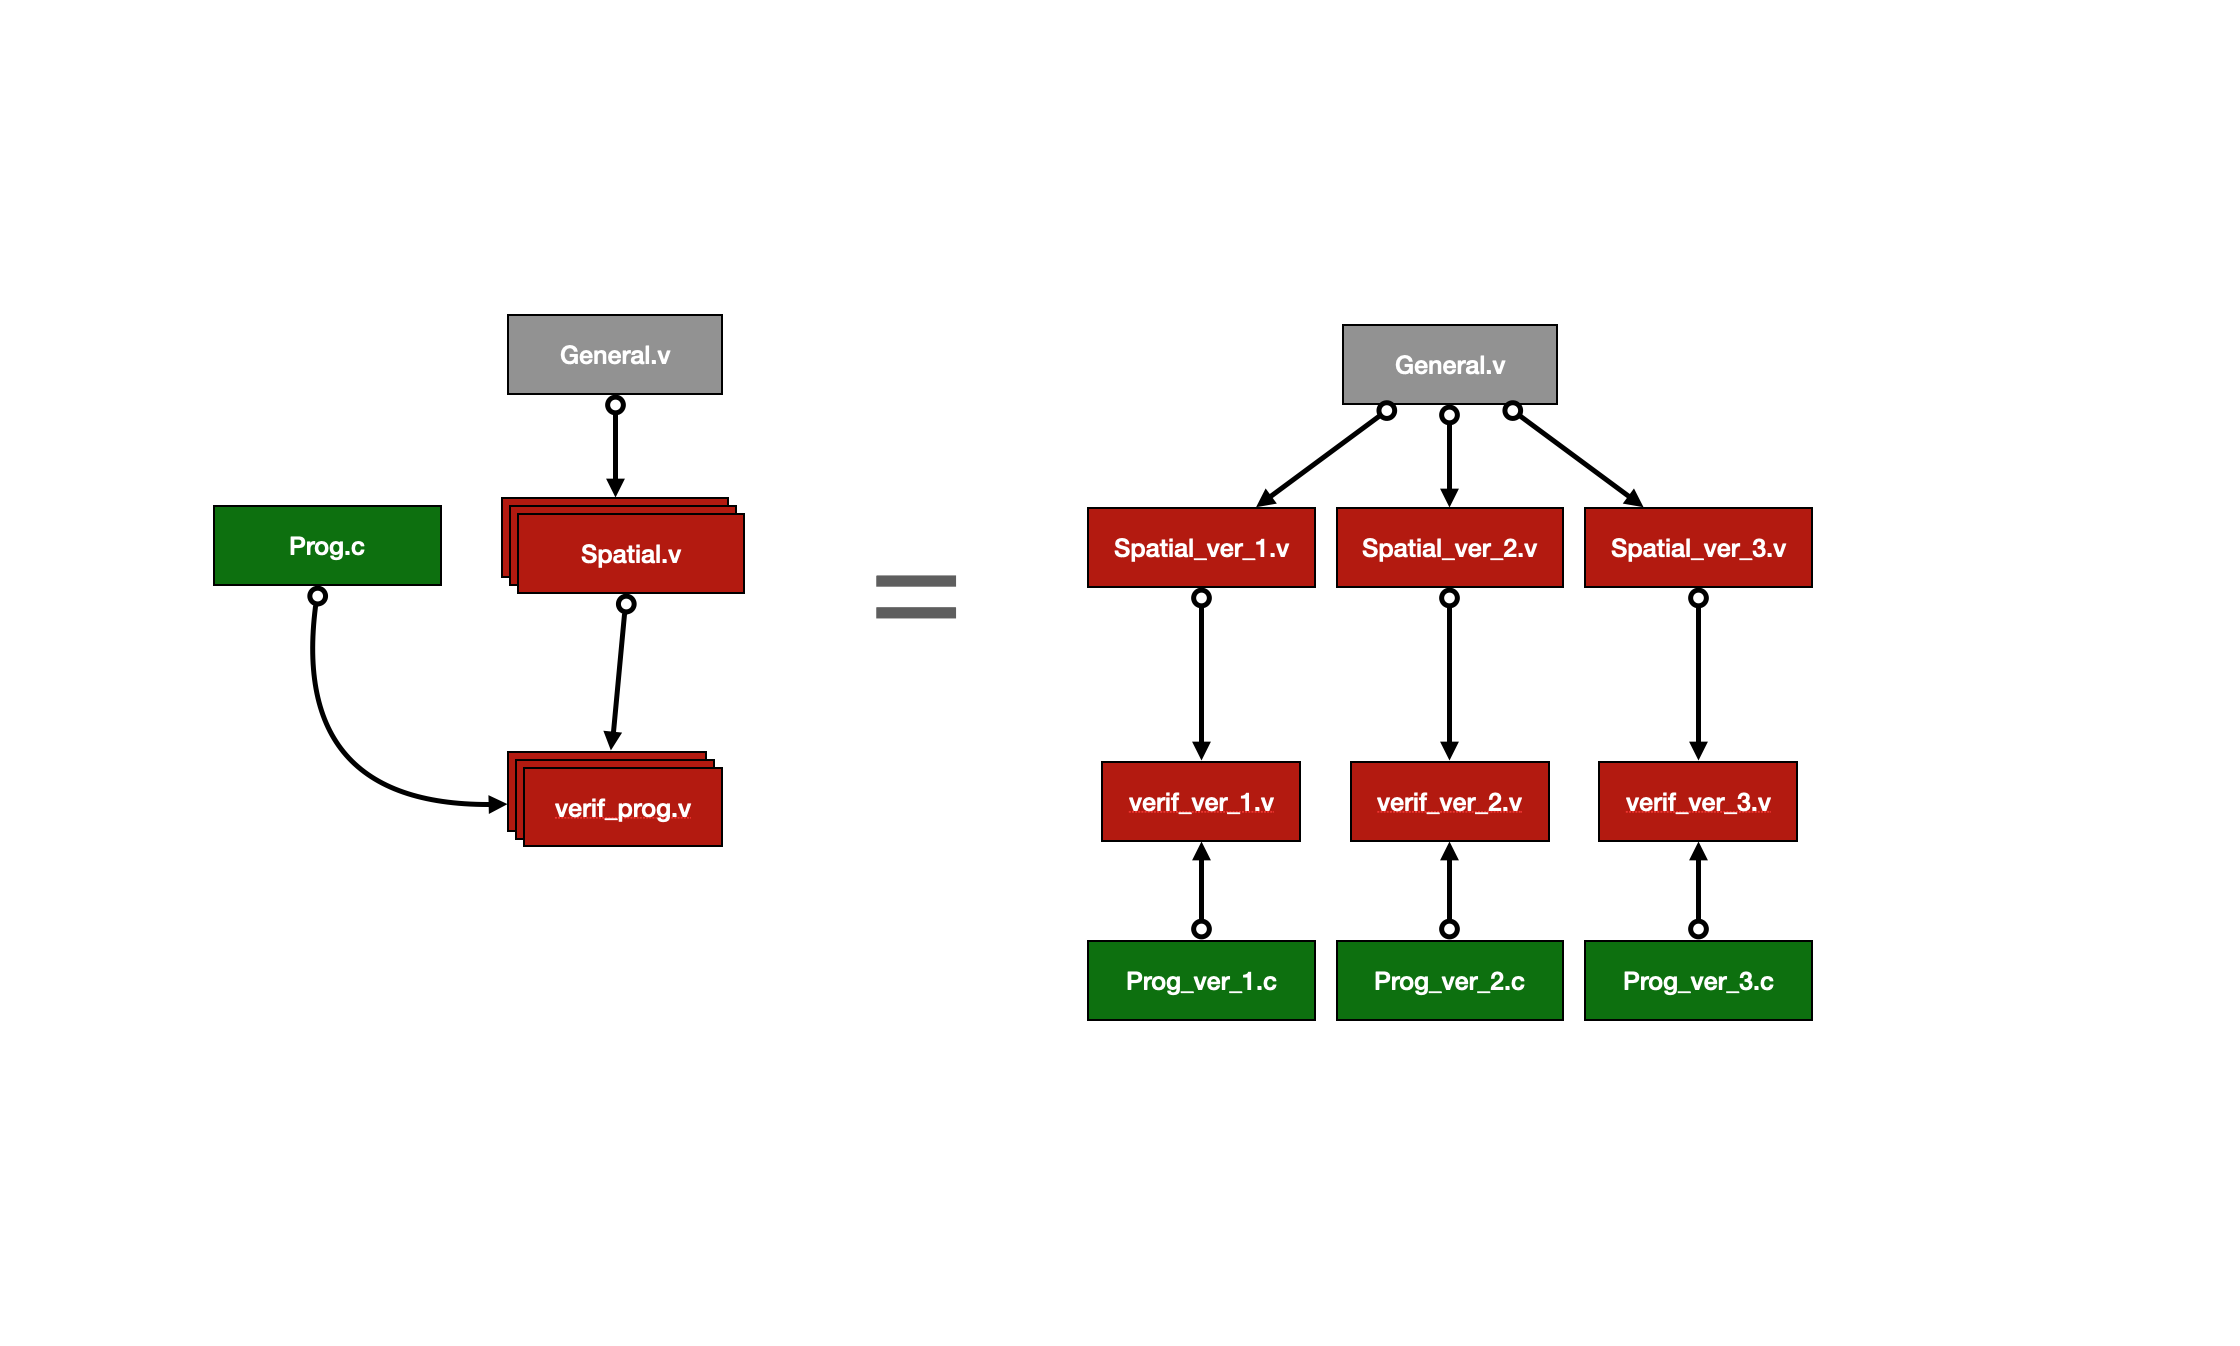
\includegraphics[scale=0.33]{key}
\end{frame}

\begin{frame}{A Note on Modularity}
\centering
  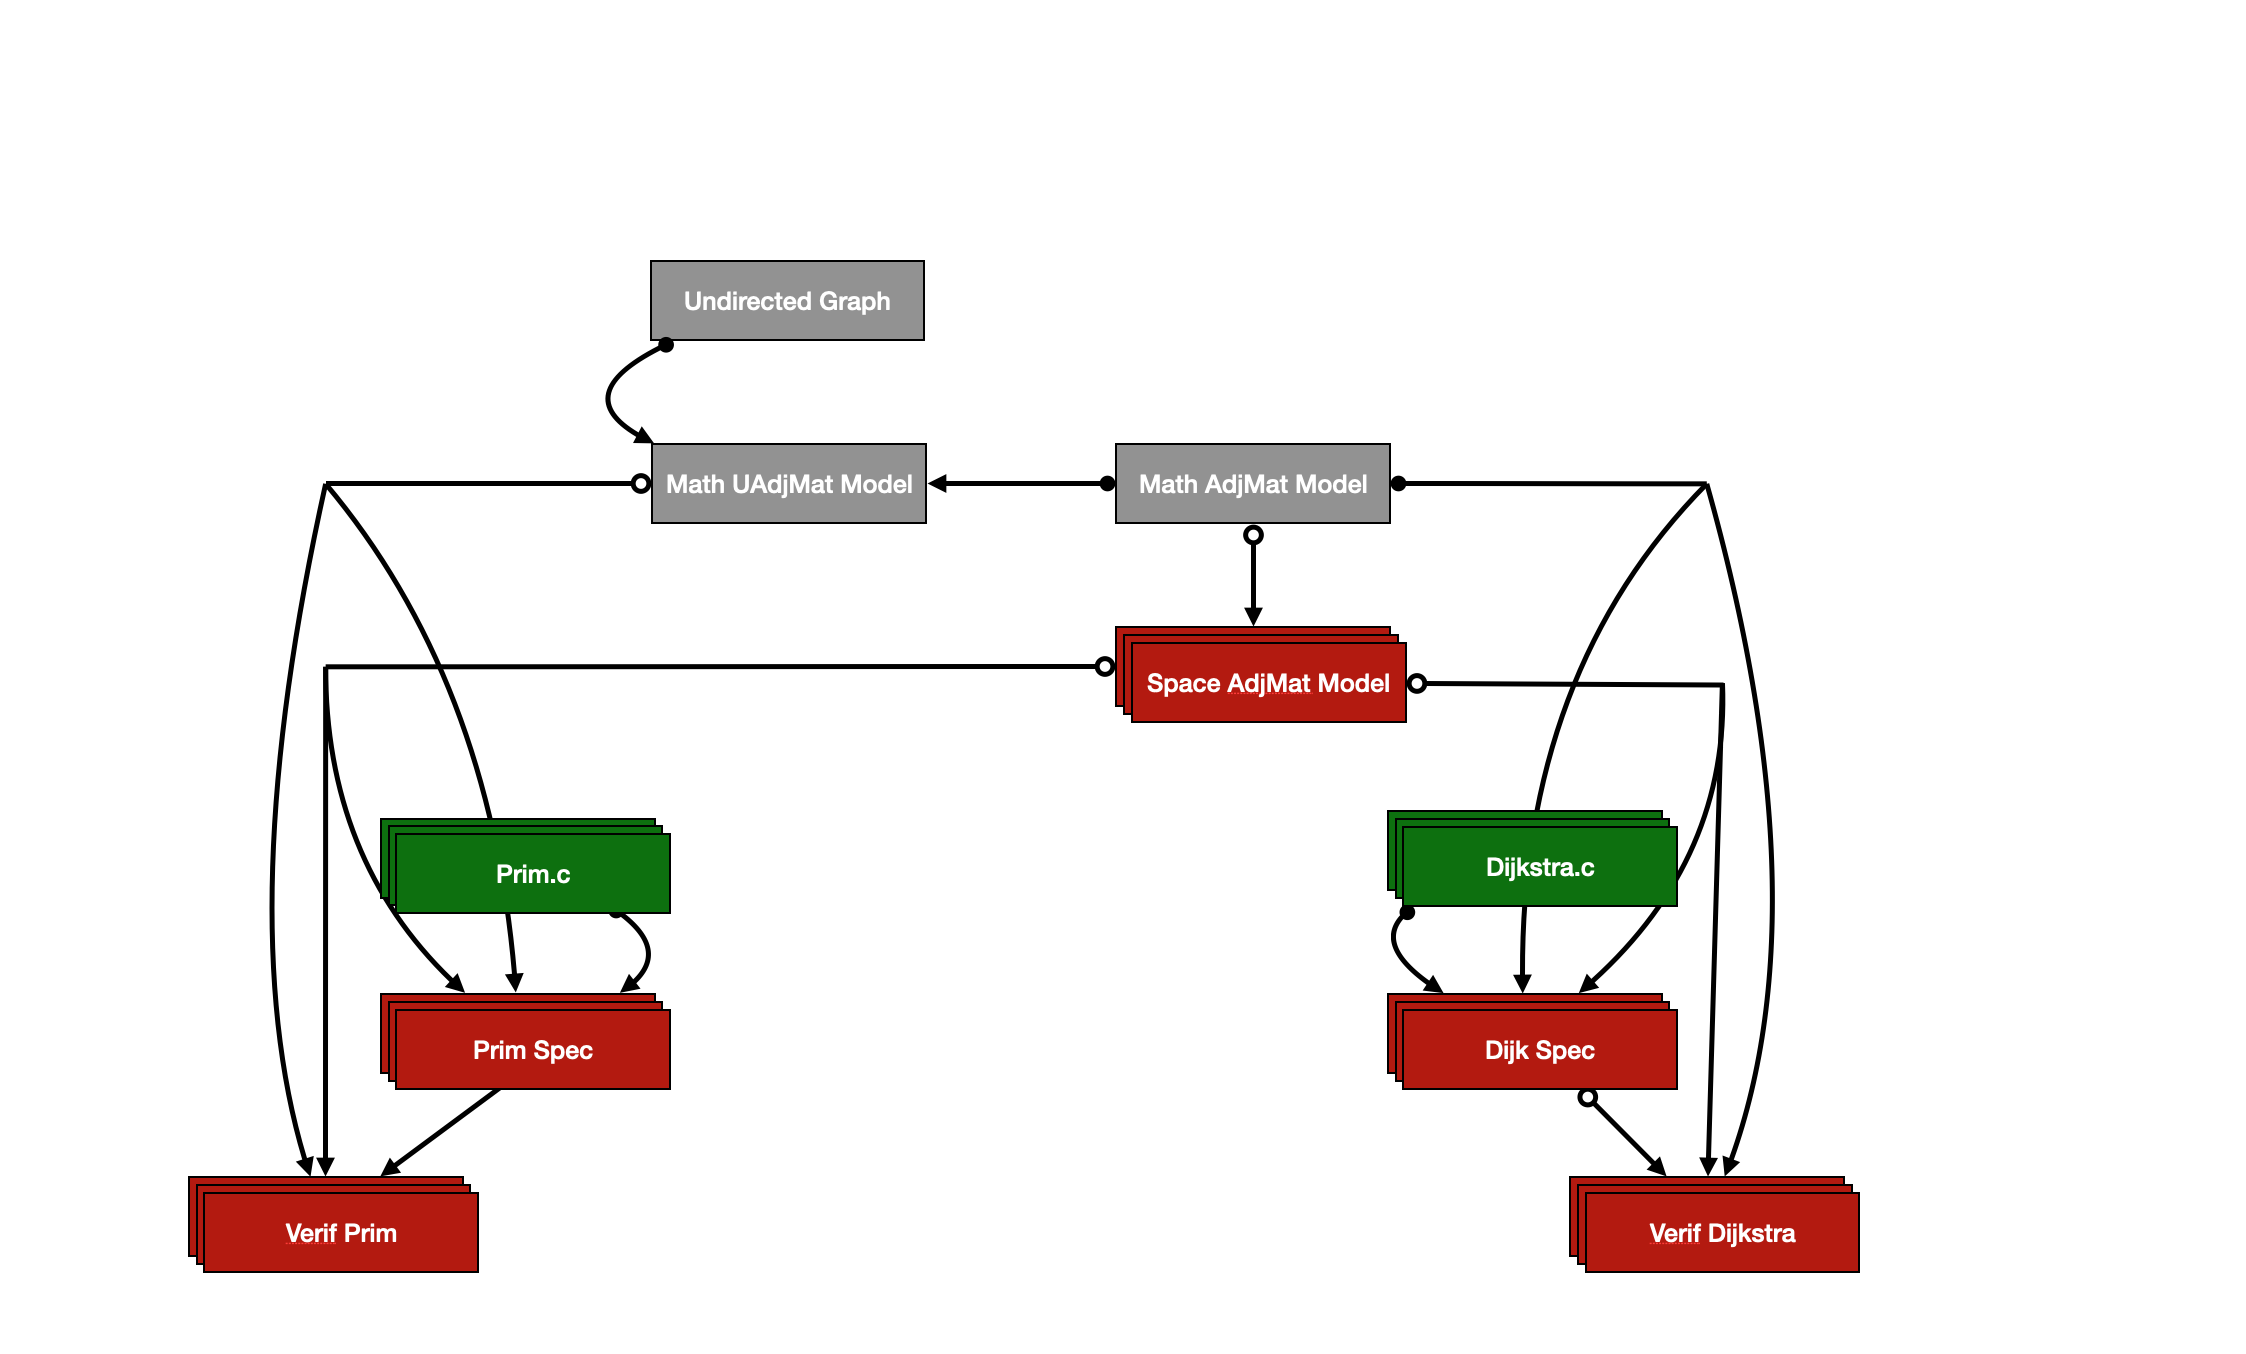
\includegraphics[scale=0.33]{simple}
\end{frame}

\begin{frame}{A Note on Modularity}
\centering
  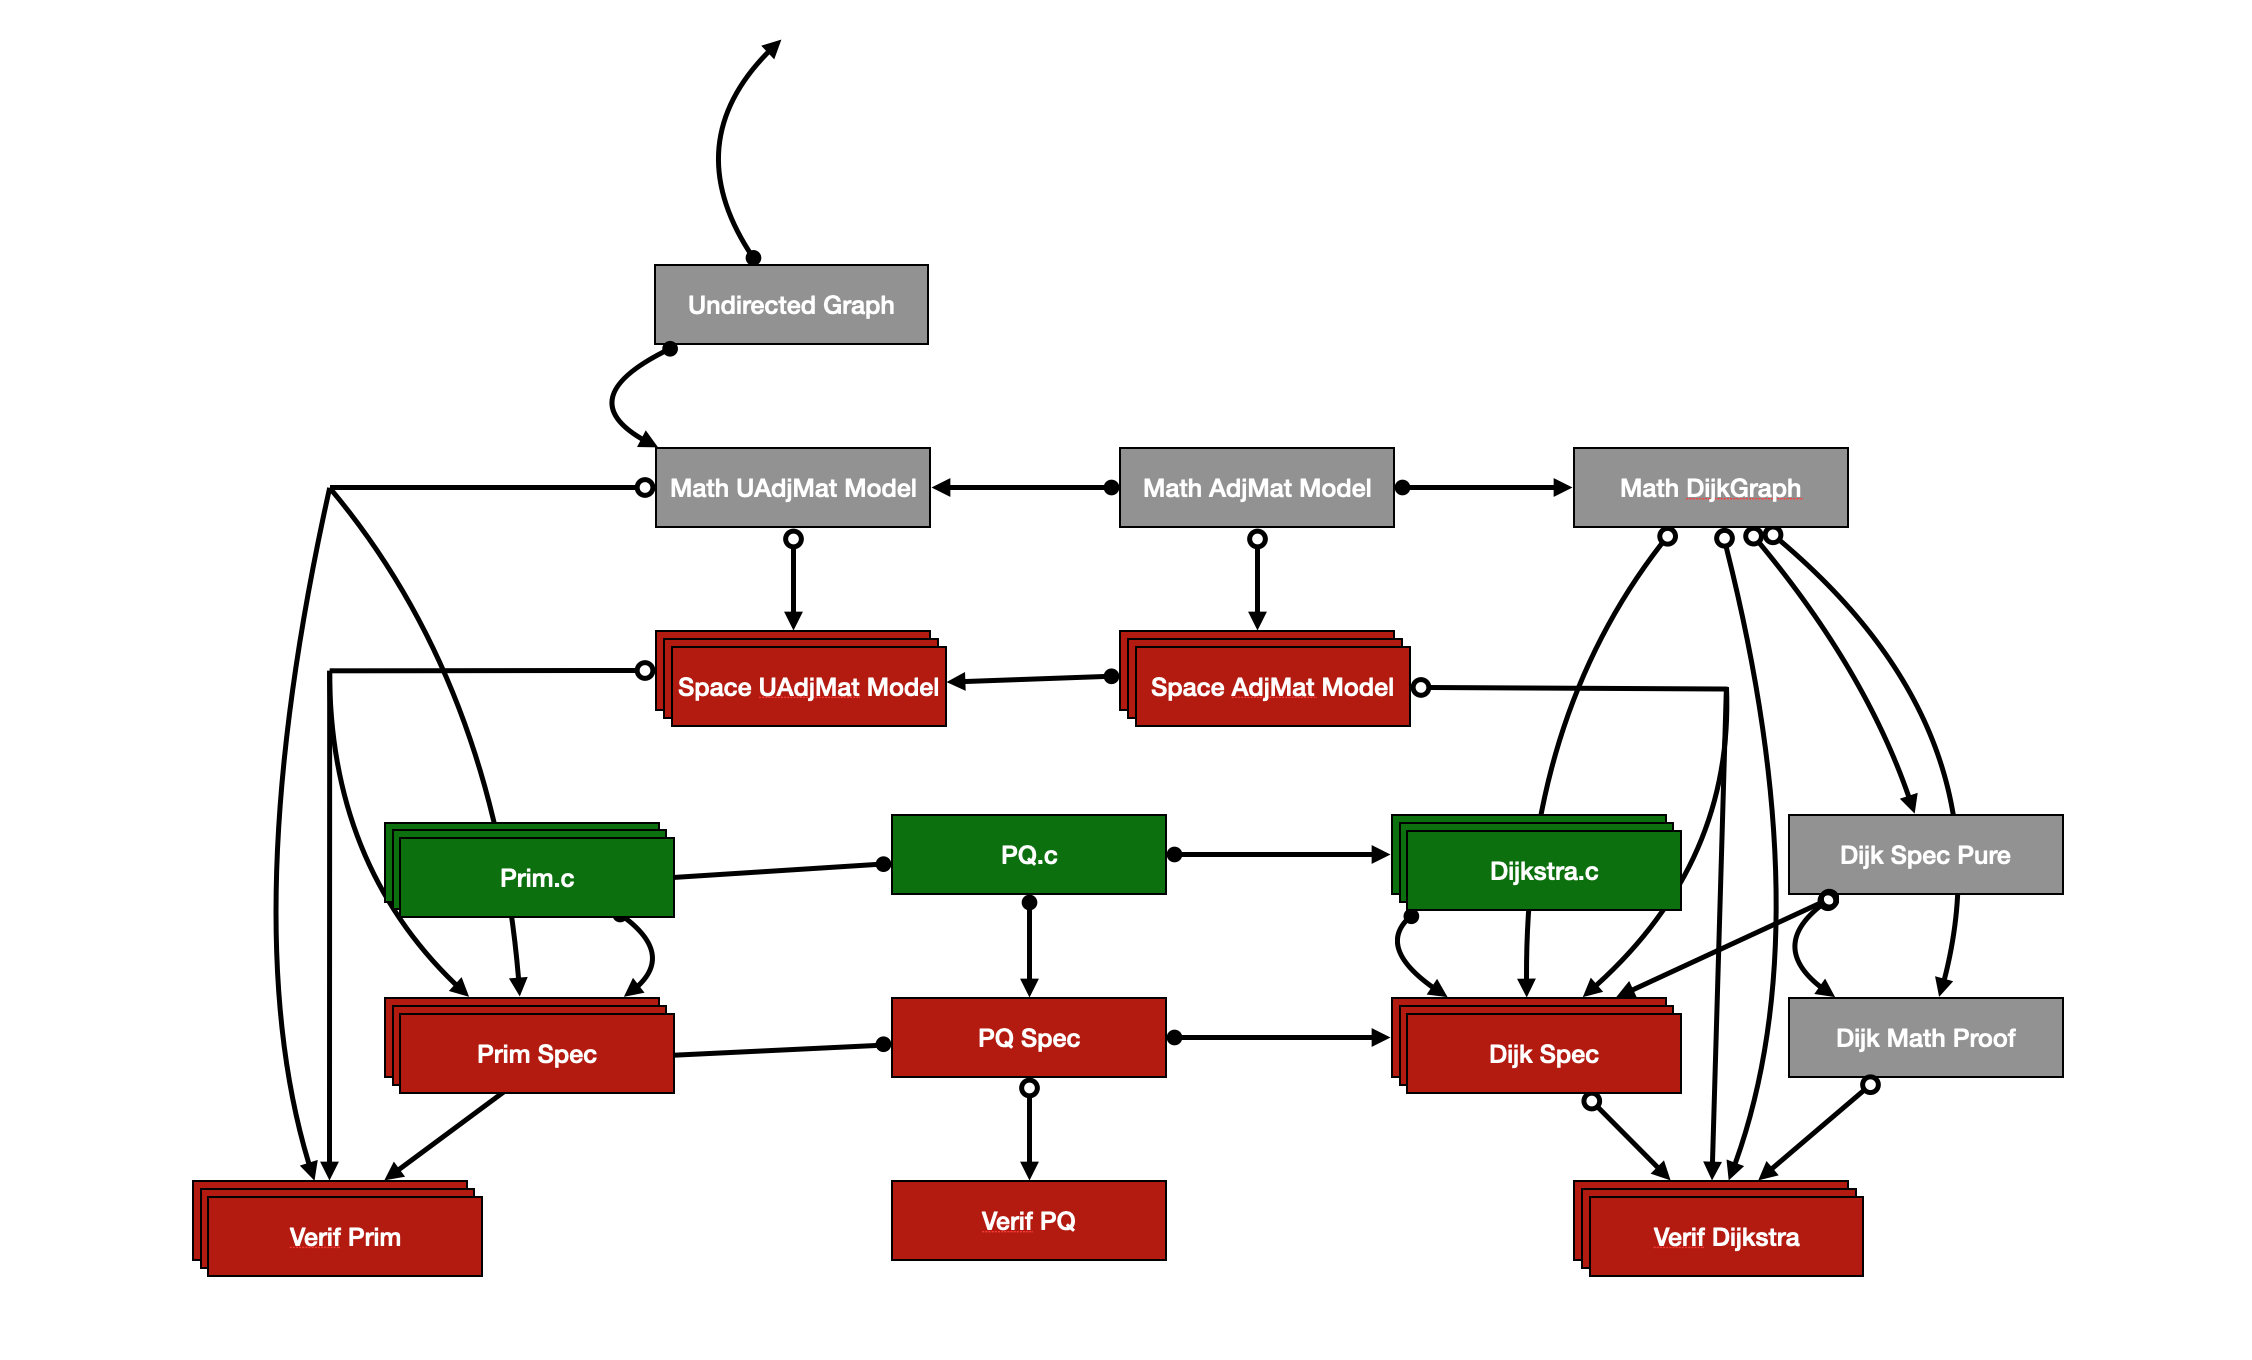
\includegraphics[scale=0.33]{dijk_prim}
\end{frame}

\begin{frame}{A Note on Modularity}
\centering
  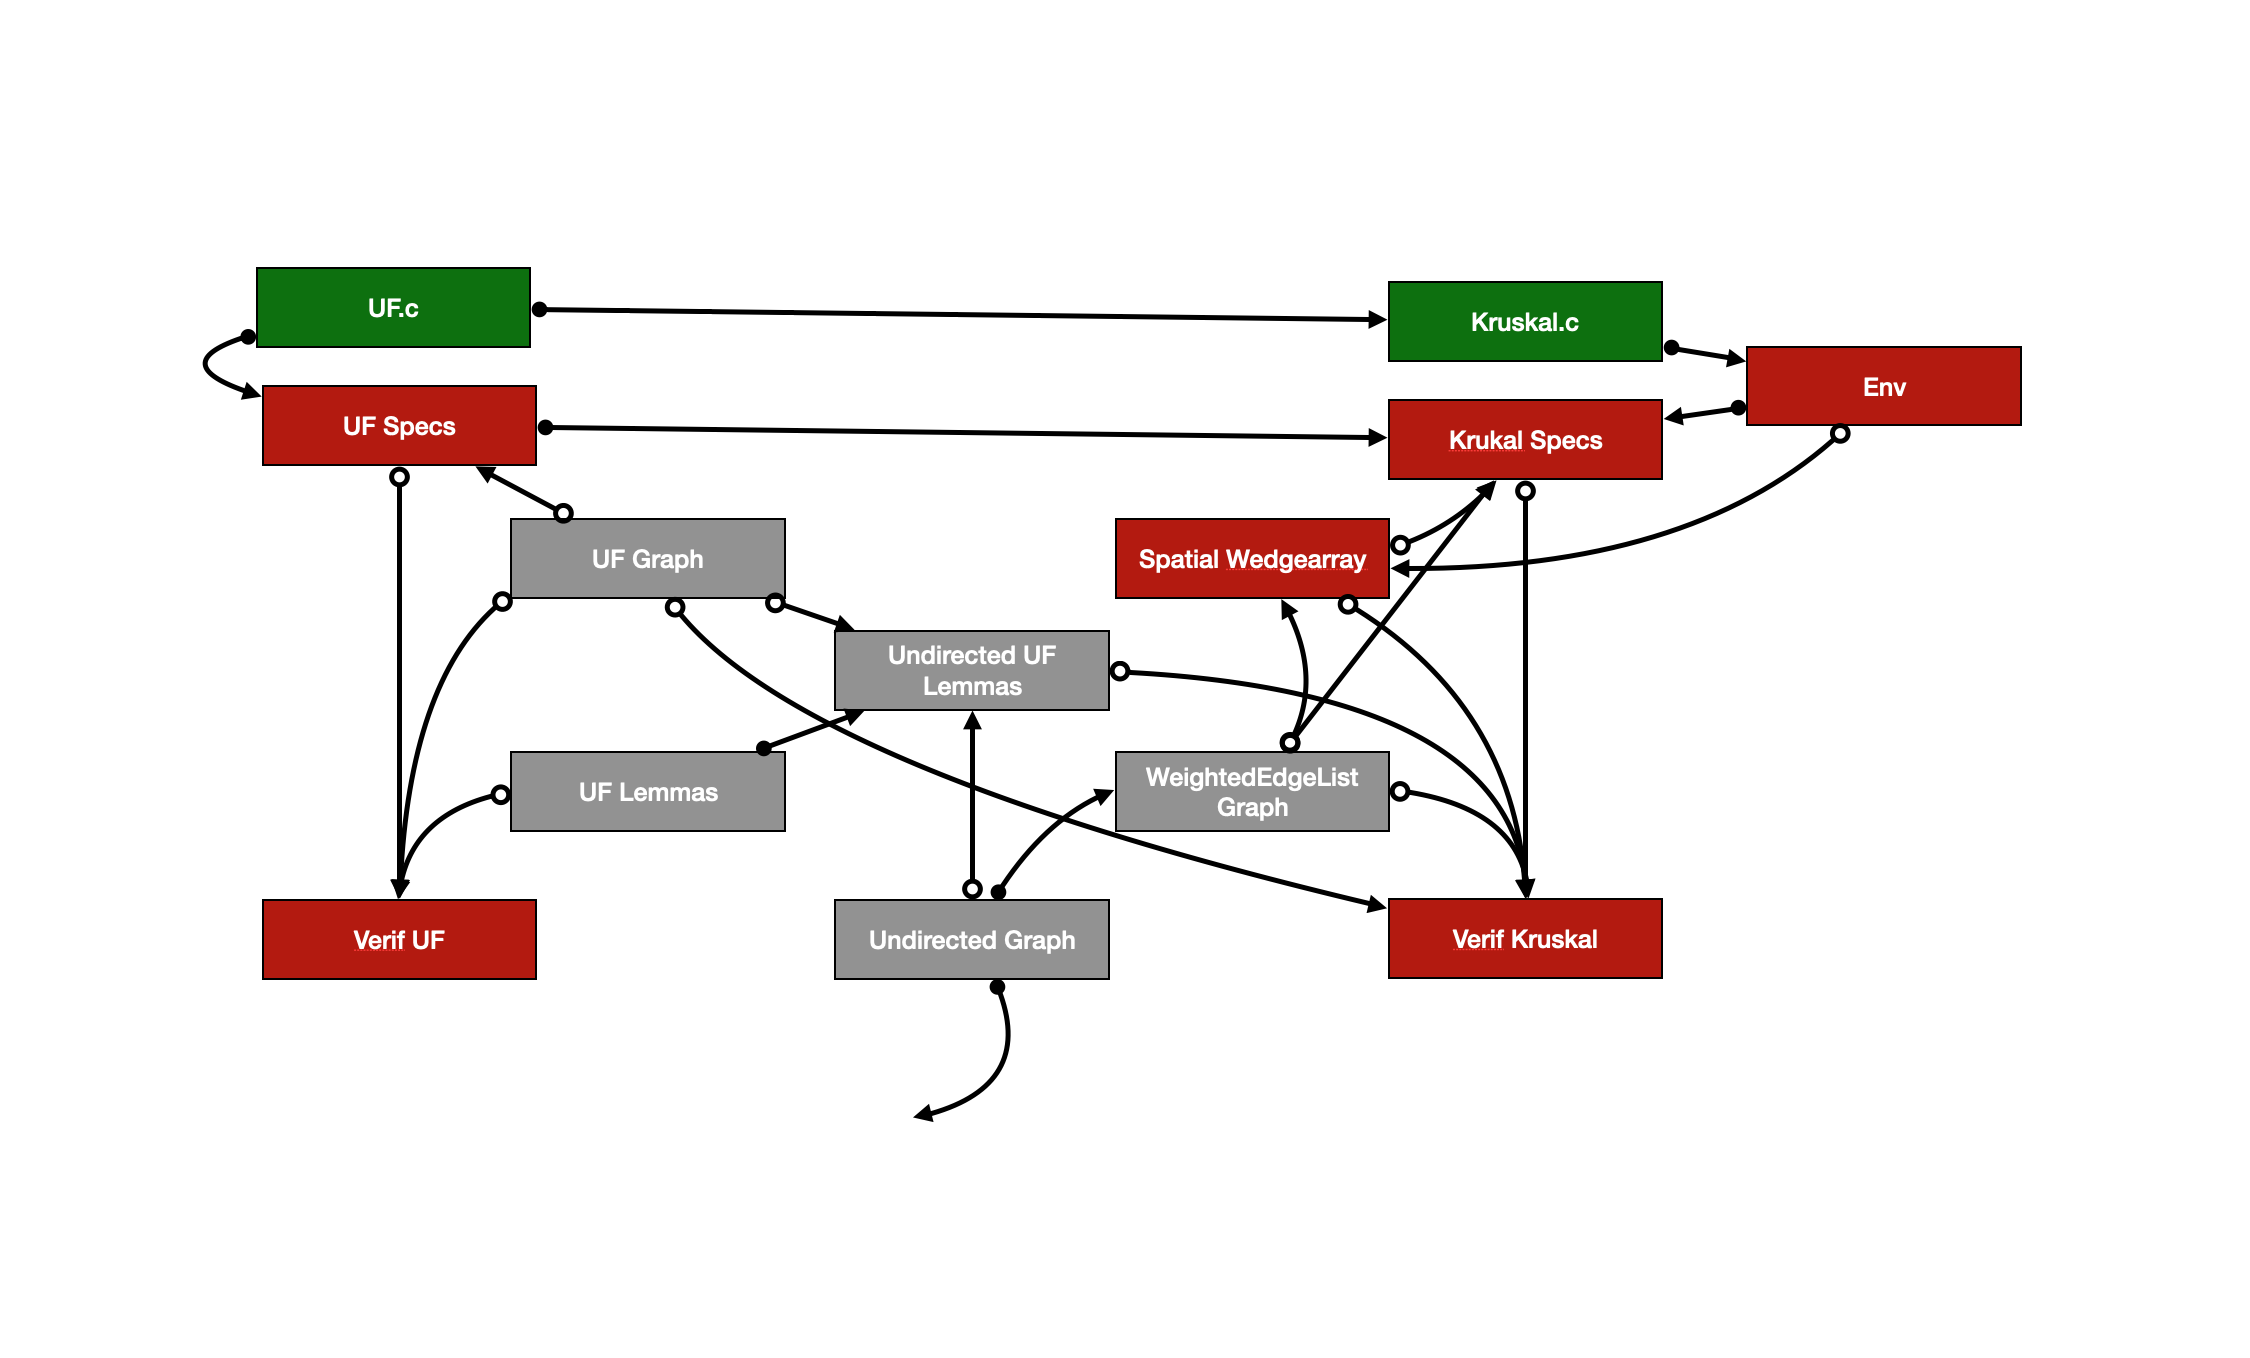
\includegraphics[scale=0.33]{krus}
\end{frame}

\begin{frame}{Possible Next Steps}
Verify PQ with \texttt{decrease-key} \\
AdjList representation for Dijkstra, Prim \\
Plug into verified \texttt{malloc} \\
Floyd-Warshall using AdjMat \\
Bellman-Ford using EdgeList \\

\flushright \pause
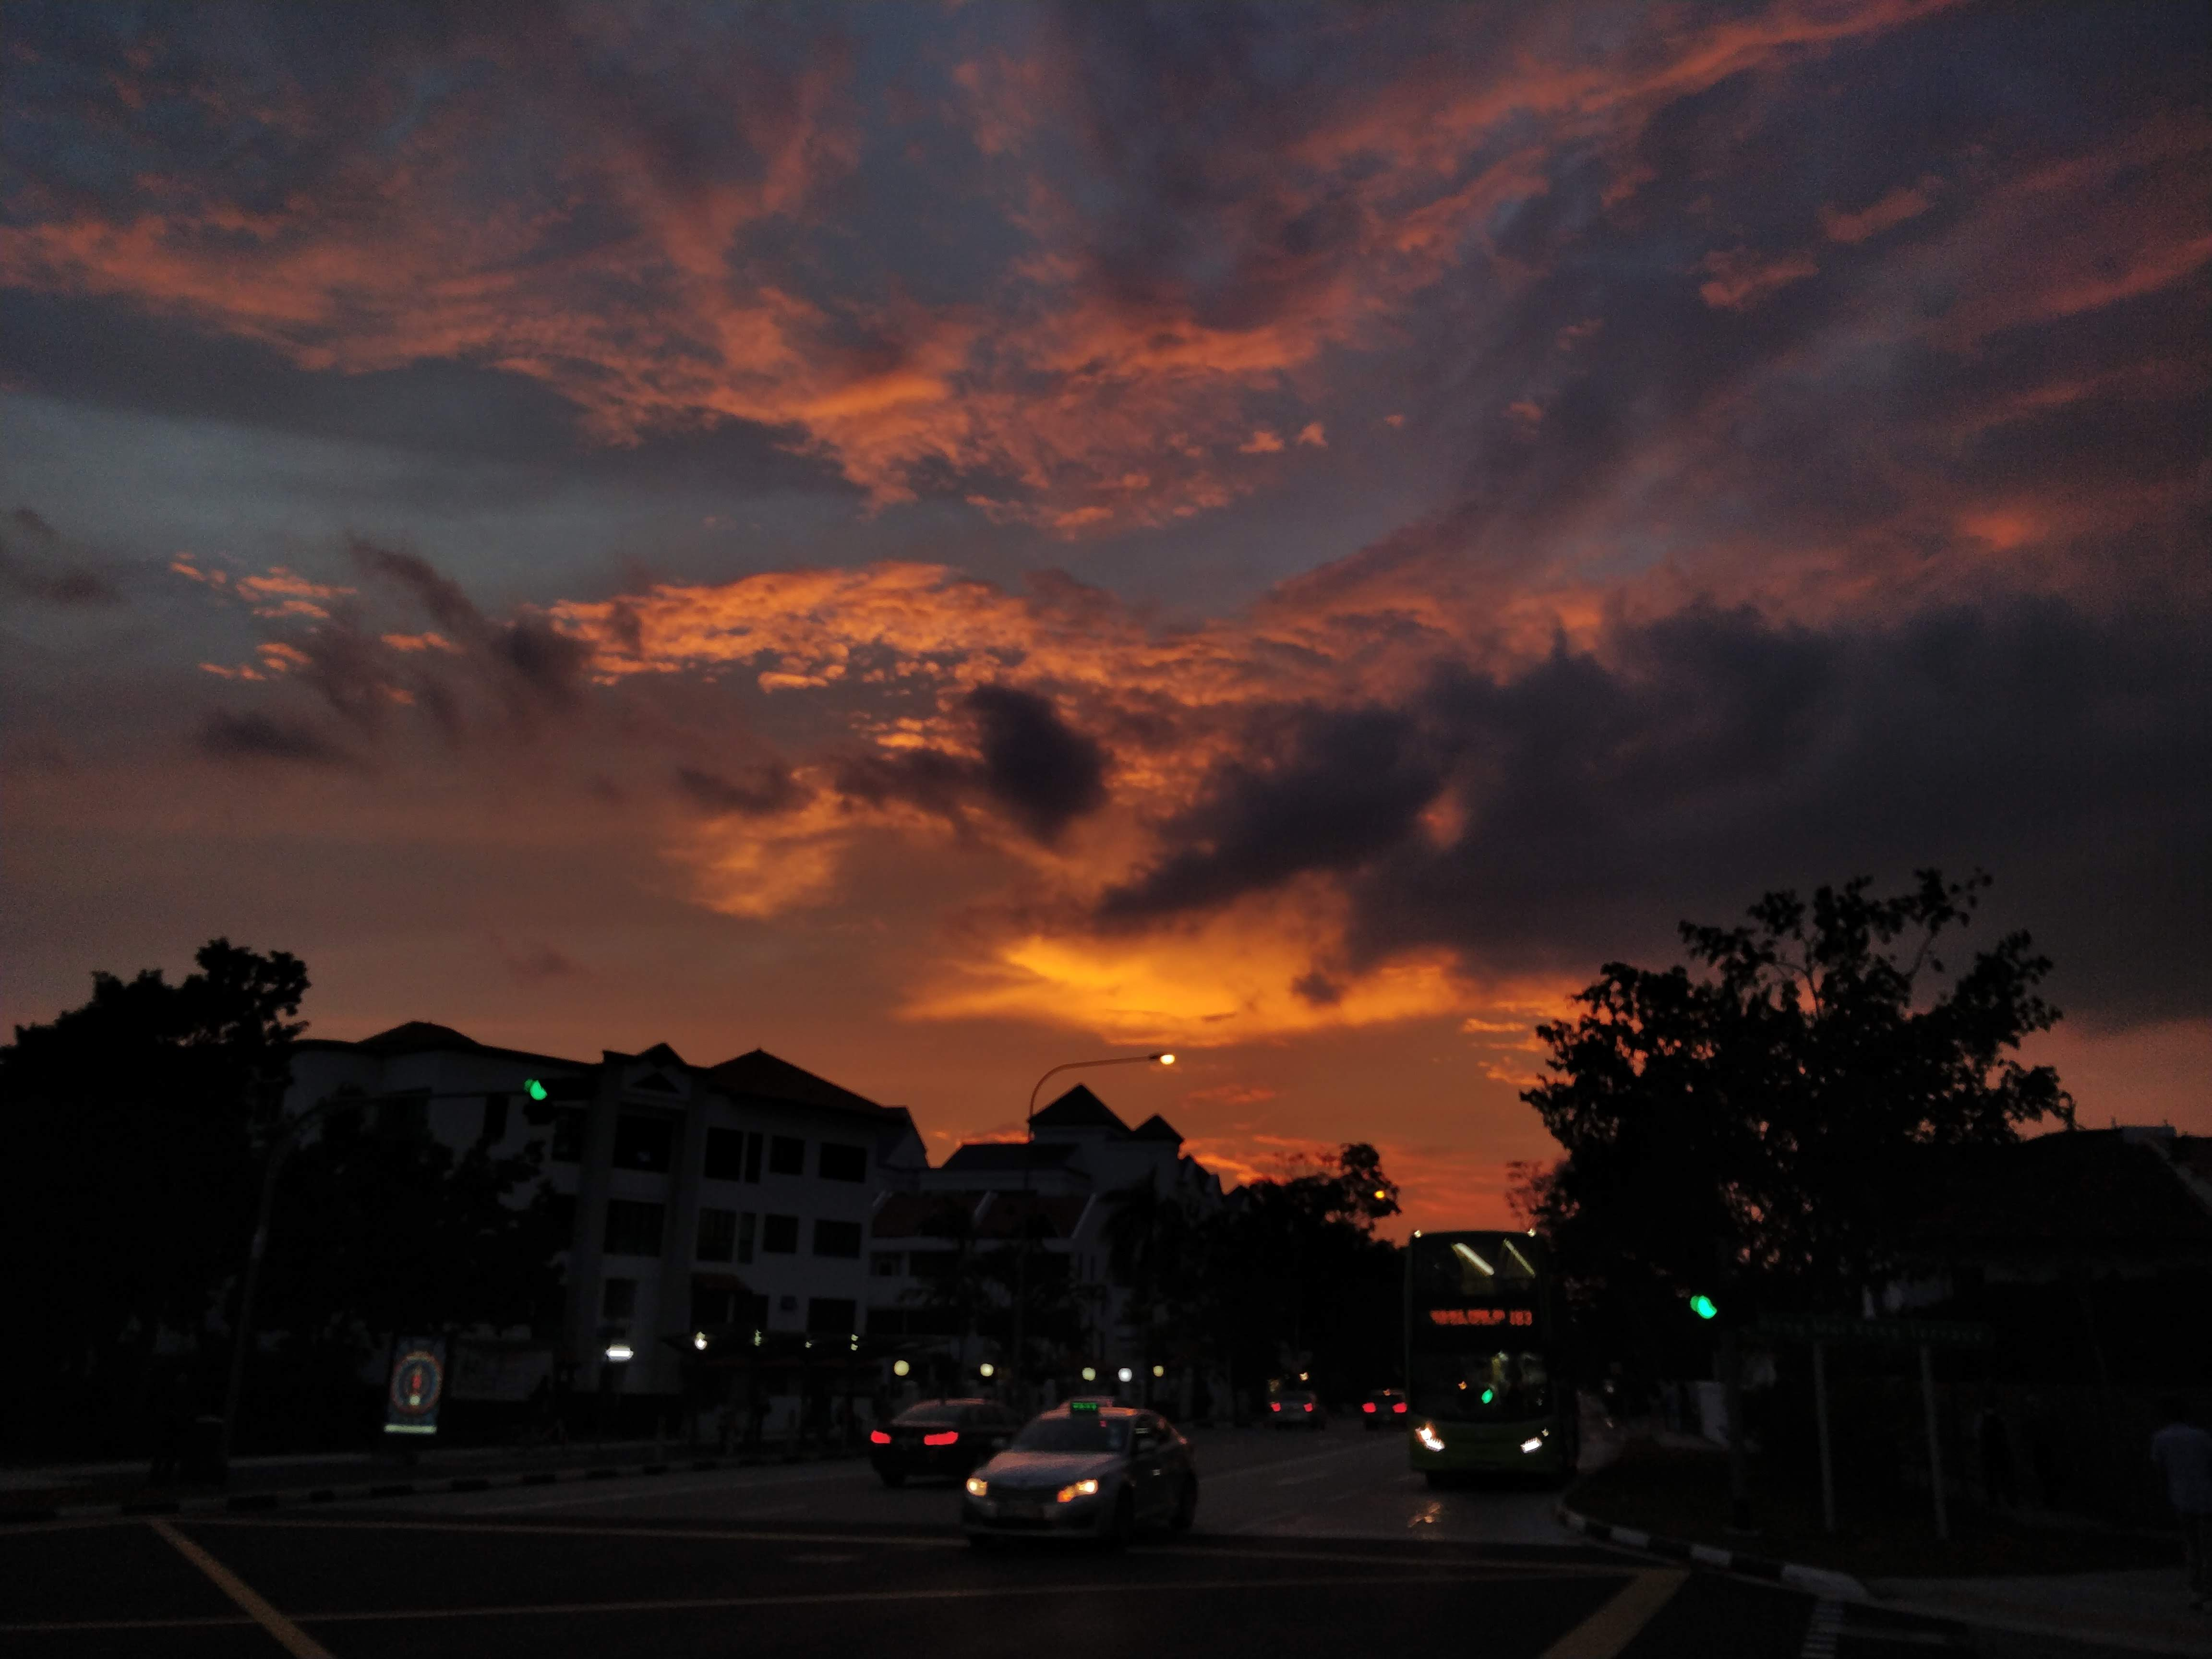
\includegraphics[scale=0.035]{sunset} \\
\vspace{-2em}{\color{white}Thanks!}\hspace{1em}
\end{frame}
\end{document}
